\chapter{Background}
\label{cha:background}

In order to understand how and why heterogeneous systems can be applied to the problem of
bitcoin mining, it is first important to obtain an understanding of how the bitcoin currency
works and what heterogeneous computing is.

\section{The Bitcoin Currency}
\label{sec:bitcoins}
Bitcoin, often abbreviated BTC, is a digital currency, using a peer-to-peer network to provide
a decentralized currency, not relying on banks or financial institutions to process transactions
or maintain accounts. An account simply consists of a cryptographic keypair, which is used to sign
and verify transactions, and as such anyone can create as many accounts as they wish. The bitcoin
project provides a variety of software for interacting with the bitcoin network and managing
accounts.

At the core of the bitcoin system is the block chain, a distributed, linked list consisting of blocks
which contains the transactions that have been executed on the network since the previous block was
generated.

A block is only valid if the arithmetic value of the double SHA-256 hash of its header is below
a certain target value. Finding a block that has such a header is computing intensive because it
has to be done through a brute-force search, and this prevents the network from being flooded with
new blocks. The target value is decided by the network ``difficulty''
and is set to such a value that, on average, six new blocks are generated per hour.

To get people to participate in creating new blocks, a reward is offered to whomever manages to
create a block. This reward also ensures that more money is added into circulation. The size of
the reward decreases over time until a predetermined number of bitcoins have entered circulation.
The reward is currently 25 bitcoins and halves every 210~000 blocks. The total number of bitcoins
that is to be generated is 21~000~000 bitcoins. \cite{bitcoin}

\subsection{Mining Bitcoins}
\label{sec:bitcoin-mining}

The process of creating a new block for the bitcoin blockchain is often referred to as \textit{mining},
refering to the fact that a lot of energy may need to be expended in order to find a valid block.

The process begins with the creation of a transaction that transfers the reward for generating the block
into the account of the miner. This transaction is often called the coinbase or generation transaction.
All transactions transmitted to the bitcoin network since the last block was generated are gathered and
the hash of each transaction is inserted into a merkle tree.

The root of the merkle tree is inserted into the header for the new block together with the hash of the
previous block and various other fields specified by the standard. If the hash of the header is below the
target value, the block is successfully mined and transmitted to the network. If the hash does not satisfy
the demands of the network, a 32-bit field in the block header, called the \textit{nonce}, can be changed
to produce a new hash. In addition, transactions can be excluded in order to produce a different merkle
root for the header.

If more than one new block is pushed to the network at about the same time, the block chain diverges.
This situtation is resolved when the next block is generated; the longest block chain is then accepted
as the canonical block chain. \cite{bitcoin}

\subsection{Pooled Bitcoin Mining}

Because an increasing amount of computing power is being used to mine bitcoins, the difficulty of finding
a block has increased to such a level that no single bitcoin miner can hope to find a block on his or her
own. Figure \ref{fig:difficulty} illustrates how the difficulty level have risen on the bitcoin network
since the beginning. The current total hashing rate is about 396,5~EH/s\footnote{$396,5\cdot 10^{18}$ H/s} according to the
statistics available from \texttt{blockchain.info}. This means that the amount of work one can expect to
do in order to find a block is, on average, 237,9~ZH\footnote{$237,9\cdot 10^{21}$ hashes}! Using, for instance,
a GPU-based bitcoin miner with a hashrate of 1~GH/s, it would take, on average, $237,9\cdot 10^{14}$ seconds,
or 7~543~759 years to find a block.

\begin{figure}[htb]
    \centering
    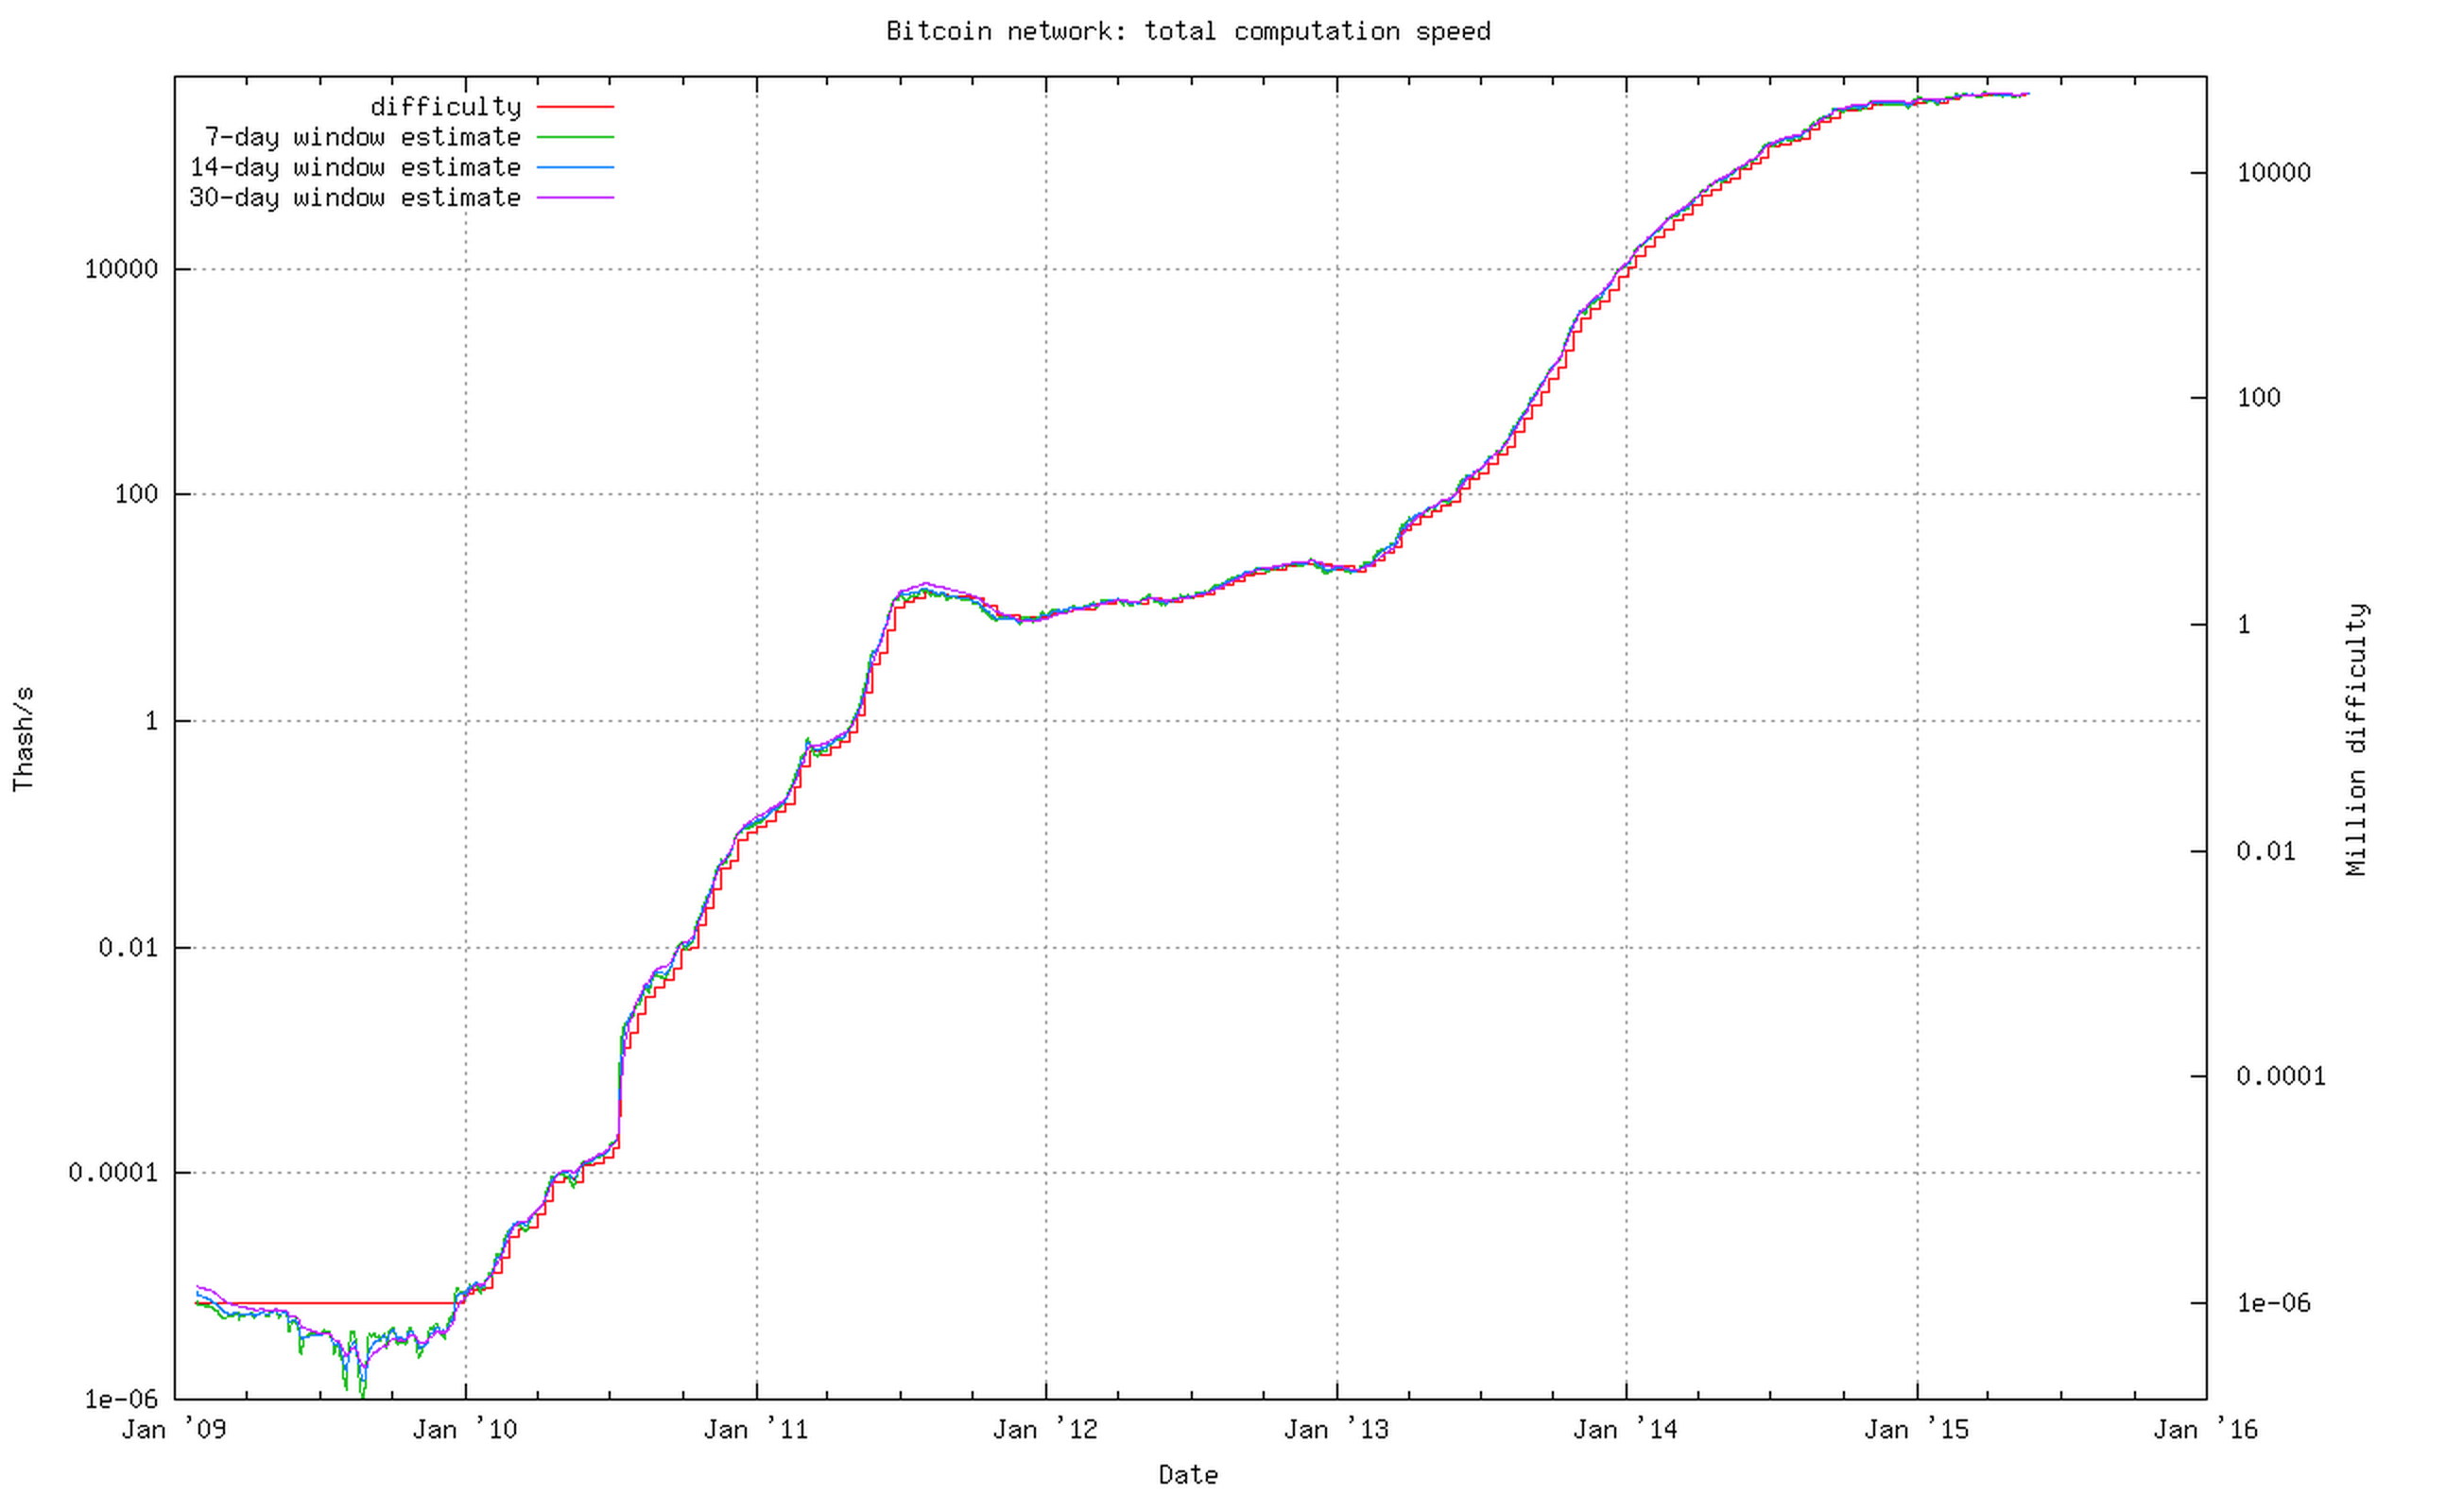
\includegraphics[width=0.95\textwidth]{Figures/Bitcoin/Difficulty-all}
    \caption{The BTC Mining Difficulty, overall history from beginning until today.}
    \label{fig:difficulty}
\end{figure}

To overcome this problem, mining pools were invented. A bitcoin mining pool is a service that distributes
work between miners. The work that is distributed has a lower target value than does the bitcoin network
itself, meaning that each participating miner can find valid blocks faster. Although most of the blocks
submitted to a pool does not fulfill the network requirements, sometimes a block does fulfill both the
pools difficulty requirements as well as the network requirements; in that case the new block is
submitted to the bitcoin network and all the miners who submitted work towards finding the block
is rewarded according to their contribution.

As such, pooled mining lets anyone with weaker hardware participate in bitcoin mining in exchange for
a smaller reward. However, using hardware such as regular CPUs and GPUs is still considered unprofitable
because of these processors' relative performance in comparison with specialized bitcoin mining ASICs.

\section{The SHA-256 Hash Algorithm}

The SHA-256 hash algorithm is defined in \cite{fips180-4} and is a member of the SHA-2
family of hash functions. Like all hash functions, it works by accepting an arbitrary
amount of input data and producing a constant-length output. The function is one-way,
that is, given a hash, it is impossible to determine the input data used to produce
the hash.

The SHA-256 algorithm works on blocks of 512~bits. Each block is split into an expanded
block of 2048 words using a message expansion function. Then each extended block is run
64 times through the SHA-256 compression algorithm, which uses simple bitwise functions
such as shifts, rotations, logic functions and unsigned addition to create a 256~bit
output value. Each round uses the output from the previous round as an initial value,
which is then combined with input data from the expanded message block.

After 64 iterations of the compression function, the result is added to the intermediate
hash values from any previous blocks, or, if there are no previous blocks, the initial
value, producing a finished hash.

A more detailed description of the algorithm can be found in appendix \ref{app:hashing-algo}.

In the bitcoin system, a double SHA-256 algorithm is used. To obtain a double hash, the
output of a previous SHA-256 calculation is simply used as input data to the hashing
algorithm.

% Is this too little or too vague?

\section{History of Bitcoin Mining}

Because of bitcoins popularity and the competitiveness involved in mining it, there exists
many different accelerators to improve the performance and energy efficiency of mining systems.
During the currency's history, hardware for bitcoin mining has evolved from regular, general-purpose
CPUs to highly specialized ASIC chips.

The bitcoin blockchain was started on January 3rd, 2009. At this point, all mining was done
using CPU mining. The official bitcoin network client supports mining and was used for this
purpose. The fastest CPU miner, a high-end, overclocked Core i7 990x eventually reached 33~MH/s
using SIMD extensions in order to improve performance. \cite{bitcoin-history}

\subsection{GPU Mining}
The shift to GPU mining started in July 2010, when the first OpenCL miner was written and
used in a private mining setup. In September that year, the first open source GPU miner
was released after the author was paid 10~000 bitcoins, worth about \$600 USD at the time,
by Jeff Garzik, one of the core bitcoin developers. An open source OpenCL-based miner was
released shortly after \cite{bitcoin-history}.

OpenCL miners typically computes the double SHA256 hash using a fully unrolled implementation
of the compression loop. Multiple calculations are run simultaneously exploiting the parallelism
offered by GPUs. Many miners tweaked parameters of their hardware, such as the voltage and
clock frequencies of both the video RAM and the GPU core in order to get higher throughput
and thus reduce the cost of running each GPU, in order to obtain greater profits \cite{bespoke-silicon}.

\subsection{FPGA Mining}

FPGA miners appeared in June 2011, providing better power efficiency as compared to GPUs \cite{bespoke-silicon}.
Early designs were mostly based on the Spartan 6 FPGAs from Xilinx, and could provide a
performance of between 200~MH/s and 220~MH/s per chip, about the same as contemporary GPUs \cite{bitcoin-hardware-cmp}
but consuming as little as a fifth of the power used by their GPU counterparts \cite{bespoke-silicon}.

% Note: Taylor managed to get the release year of the GPUs he compares performance to wrong,
% choosing GPUs from 2012 to compare to FPGAs from 2011.

FPGAs provided great advantages to the speed of bitwise functions, which are important for
the SHA256 algorithm. Popular open-source designs were created so that they could be used
by different kinds of FPGAs. They consisted of a SHA-256 module which could be configured
with a specific unroll factor, that is, they had a configurable depth pipeline, each
consisting of the neccessary hardware for computing a specific number of rounds of the
SHA256 compression function. Completely unrolling the algorithm created a pipeline of
64 stages, with a throughput of 1 hash per cycle, while it was also possible to specify
lesser unroll factors which resulted in fewer pipeline stages and reduced throughput, taking
several cycles to perform a hash but saving registers and logic resources in the FPGAs.
The pipelines were duplicated to improve performance.

Power consumption became much higher than typical for FPGAs, with the pipelined design
giving extremely high activity factor for LUTs. Pre-made boards could not provice enough
power nor heat dissipation to sustained usage, and hackers thus developed custom
boards that focused on providing enough power and cooling with minimal unused resources,
such as RAM and I/O components. \cite{bespoke-silicon}

\subsection{ASIC Miners}

Neither GPUs nor GPUs can compare to ASICs, specialized chips that started to appear on the network
in the beginning of 2013 \cite{first-asic-miner}. It was the need for more high-performance and power
efficient bitcoin miners caused implementors of bitcoin miners to turn to ASIC solutions.

One of the first ASIC designs were Butterfly Labs' ASIC miners. Having experience developing
FPGA based mining solutions, the company created an ASIC chip with 16 double SHA256 modules,
the equivalent of 16 FPGA-based miners using a 65~nm process. The end-product ended up being
delayed when the chips ended up consuming more power than expected and had to be underclocked
in order to be able to cool the chips properly.

ASICMINER was another of the earliest designs, including only one SHA256 hash unit on a chip,
replicating a single FPGA-based design at a much higher frequency, with better power efficiency
and a cheaper price. \cite{bespoke-silicon}

\subsubsection{The Goldstrike 1}
Another ASIC design is the Goldstrike 1 architecture, noteworthy because its architecture is
described in an article in IEEE Micro. Because of the competitive nature of bitcoin mining,
it is not common for designers of ASIC solutions to reveal too many details about the architecture
of their chips and few scientifi papers exist on the topic.

The Golstrike is an ASIC-based bitcoin mining solution capable of reaching 2~TH/s. To reach the performance
requirements, a bitcoin mining core was created that was able to perform at 125 GH/s. Four of
these were combined in one package, with four of these packages then combined on a circuit board
to produce the target performance.

The Goldstrike cores consist of an architecture with 120 hash engines running in parallel.
A hash engine searches through all possible values of the 32-bit nonce field in the bitcoin header
(see section \ref{sec:bitcoin-mining}) in order to find a valid hash.

The hash engines uses a pipelined double-SHA256 implementation, with each round of the hash calculation
unrolled into a pipeline.

Tinished ASIC chips, each with four bitcoin mining cores, was measured to provide 504~GH/s while using
500~W of power. This gives a power efficiency of about 1~GH/J.

Interestingly, the architecture provided challenges when it comes to powering and cooling the chips.
Because the architecture uses all available computing power for bitcoin mining all the time while
the chips are in use, no parts of the chips can be turned off to save power. \cite{goldstrike}

% Fun fact, GH/Ws = GH/J

\subsection{Scaling of bitcoin hardware}
Due to the dark silicon problem, future chips will require that parts of it must be powered down or deactivated,
in order to satisfy a given power budget\cite{dark-silicon2}. As mentioned, bitcoin mining may be close to
the worst case for dark silicon optimizations, far beyond multicore CPUs or GPUs. Due to bitcoin mining's high procesing requirements, the logic needed to run the algorithm cannot be turned off without losing
performance.

BLF ran into this problem with their 65~nm chip, and had to scale back the performance to reduce power consumtion
and manage to cool the chip properly. While bitcoin mining began as a ``race to ASIC'', energy costs now determines
which ASICs are the most profitable and thus energy efficiency is a problem that must be addressed. \cite{bespoke-silicon}

%\section{History of Bitcoin Mining}
%
%\todo{Remove everything from here and move to Related work!}
%
%\subsection{CPU}
%Source code for bitcoin-mining began with the CPU, back to early \todo{Find more excact date? Perhaps with together bitcoin itself?}2010. 
%The following code found from \todo{add source: https://github.com/bitoin/bitcoin/blob/master/src/miner.cpp}\cite{bitcoin github} demonstrates the simple algorithm.      
%       
%\begin{lstlisting}%[frame=single]  
%
%while(1)
%    HDR[kNoncePos]++;
%    IF (SHA256(SHA256(HDR)) < (65535 << 208) / DIFFICULTY)
%        return;
%\end{lstlisting}
%
% COMMENTED OUT: This is already explained in Related Work and under Bitcoin Mining.

%To further optimize this code, a mid-state buffer has been taken into use.
%This buffer contains the beginning portion of the block header that precedes the nonce, and has the \todo{Make sure this constant intermadiate hash value is described earlier}constant intermediate hash value.
%For each of the 64 rounds of basic encryption, a high number of operations are involved.
%These are 32-bit additions and rotations, bit-wise functions including xors, majority, and mux-functions, and use of an array with 64 32-bit constants.
%Every operation in the 64 round encryption is dependant on the preceeding ones, making parallelization of one SHA-256 computation impossible.
%But the different rounds where trying to find a new nonce are independent of each other, and can thus be parallelized.
%
%Multicore CPUs usually have hardware optimized for less regular computations, which result in wasted performance and energy efficiency. \cite{bespoke-silicon}
%
%At the best of its time, the high-end overclocked six-core Core i7 990x eventually reached 33 MH/s when using SIMD extentions.
%
% COMMENTED OUT: Merged into Related Work

%\subsection{GPU}
%The first CUDA miner was released in September 2010, and first OpenCL miner in October 2010, which has been further optimized and adapted afterwards by different parties.
%While the bitcoin protocol itself was often implemented in another language, such as Java or Python, the mining itself was implemented through OpenCL.
%It i a single linear code region where the nonce at start is based on the thread work item id, with both chained 64 SHA256 hash rounds executed in a single unrolled loop.
%The external memory is usually not accessed in steady state, and when a successfull nonce is found, it is flagged at the end of the OpenCL routine, where the driver code will act on this. 
%
%Since GPUs were to mine for many months, the users would tweak the voltage, the video RAM operating frequencies and the core it self, in order reduce costs where possible and increase througput, balancing performance against power saving, and reduce the waste from unused parts (such as the RAM).
%Input parameters were tweaked as well, such as thread numbers, to balance maximum throughput with stability and temperature limits, and they would be retuned over time as the GPUs would wear out and cause critical paths to run slower.
%
% COMMENTED OUT: Merged into Related Work

%For the building and use of rigs, GPUs were more accesibale than FPGAs for end users, since the minimum requirement were PC-building skills and eager forum-reading.
%No formal training in parallell computing or FPGA tools were required.
%There were a few key restrictions, however, that had to be addressed and tweaked with:
%With GPUs followed additional cost in wasted resources, such as necessary motherboards needed for the GPU's, but with unused processors, hard-drive and RAM. 
%Each GPU demanded power, typically 200-300W per GPU.
%GPUs used at this scale goes beyond the airflow design of the rig cases, and the power consumption easily exceeded beyond natural cooling, power and noise limits.
%Each GPU needed to be plugged into a PCI-E 8x or 16x slot, which there were few on the commercial motherboards, and OpenCL required each to be attached to a display. 
%
%\todo{Dilemma: Have said part A, need to say part B? Or avoid it due to the excessive amount of details (vote the last)}\textbf{Dropped the GPU rig-limits solution}
%
%The power consumption on each GPU were 200 Watts or more, making the use of rigs comparable with data centers.
%For some residental homes, only one or two GPUs could be utulized before the price per KWh was jacked up for the resident.
%The most successful Bitcoin mining operations tended to relocate to warehouse space with largers volume for air for cooling, and with cheap industrial power rate.
%
%At the best of its time, NVidia GPUs like GTX570 reached 155 MH/s rates, while AMD GPUs like 7970, costing \$450, performed as much as 675 MH/s.\cite{bespoke-silicon}
%
% COMMENTED OUT: Ya

%\subsection{FPGA}
%The first open-source FPGA bitcoin miner was released in June 2011.
%The FPGAs have an edge in rotation operations and bit-level operations, but the SHA256's 32-bit addition operations were less great.
%In scaling, the designers created a single SHA-256 module that could be unrolled, specified by a parameter.
%At maximum unroll, different hardware for each of the 64 rounds of the hash were created, with pipeline registers in between, containing the running hash digest and a full copy of the 512-bit block being hashed.
%With the state for a current nonce proceeding down the pipeline, one stage per cycle, this allowed a maximum throughput of one hash per cycle.
%Alternatively, the pipeline could be reduced to calculate a hash every N cycle, while more duplicates of the pipeline could be synthesized for independent calculation in \todo{They didn't use this term in the Taylor-paper, recommend finding more sources to back up}parallell.
%Depending on the size of the FPGA, the trade-off were found between the unroll factor and duplication of the pipelines.
%
%Power consumption became much higher than typical for FPGA, with the pipeline design giving extremely high activity factor for LUTs.
%Pre-made boards could not provide enough power current nor heat dissipation to sustain usage, and hackers thus developed custom boards that focused on providing enough power and cooling, and minimalized unused resources (such as RAM and I/O).
%Using Spartan XC6SLX150 parts and placing these on quad-chip boards, they achieved a maximum of 860 MH/s at 216 MHz and 39W, at the price of \$1060.
%
%Butterfly Labs (BFL) in Kansas offered a non-open-source version, with the price of \$599 with performance at 830 MH/s.
%They also offered a higher-end Goliath FPGA-based machine, the BFL Mini-rig, with priced at \$15K that achieved 25.2 GH/s, based on Altera FPGAs that each reached 650-750 MH/s per chip.
%BLF was the most \todo{Advice: Google and check if this still stands}successfull commercial closed-source Bitcoin company.
%
%The prime benefit of using FPGAs were the energy efficiency, where the consumption were to one-fifth, compared to the best non-FPGA solutions.
%FPGAs had competition from the best GPU-solutions, however, with the FPGA being more expensive with less potential for resale, and with the GPU's better scaled silicon, down to 28-nm, vs the 45-nm of the FPGAs.
%
%FPGAs didn't last long before ASIC miners came to the market, but the design laid the foundations for ASICs, and therefore were important for the development. 
%The ASIC Verilog designs were similar to the preceeding FPGA Verilog, as well as the board, packaging and distribution infrastructure, giving already built expertize that would help in the ASIC generation.
%\cite{bespoke-silicon}
%
% COMMENTED OUT: Already merged into Related Work

%\subsection{ASIC}
%
%Butterfly Labs (BFL), ASICMINER and Avalon were the first three \todo{Not sure if 'company' is the right term}companies to provide ASIC Bitcoin miners that came to market.
%Unlike most ASIC production, these were funded by the community, either through raising money over the Internet, or by preordering by the users.
%
%The final products had delays. 
%BLF, in spite of their success and newly developed expertice with FPGA BTC miners, had several setbacks and had to scale down the final chip product from 500 MHz to 250 MHz, because power consumption ended up at 4-8 times as much as initally estimated, leading to problems with heat dissipation.
%Their products were shipped in April 2013, five months behind the initial estimation.
%ADICMINER experienced had several problems: The shutdown of GLBSD Exchange, which they used for funding and selling BTC miners, led to temporarily loss of the customer order list, and the fab had busy periods and prioritized larger companies, and demanded changes in their design, all this reducing fab throughput. 
%ASICMINER also needed to train workers to assemble the units, and aquire a warehouse space for sufficient stable power and cooling for the machines.   
%
%Finally, the end products were the following:
%\begin{description}
%    \item[BLF] 
%    Shipped in April 2013.
%    Three products: \$149 Jalapenos rated at 4.5 Gh/s, \$1299 SC Singles rated at 60 Gh/s and \$30K SC MiniRigs rated at 1500 Gh/s, all at 65-nm.
%    Compared to GPUs and given the prices, the machines were initally expected to generate 20-50 times more bitcoins per dollar, compared to GPUs.
%    Each BFL chip would contaion 16 lanes of double SHA-256 hash pipelines, making one ASIC equal to 16 Spartan-6 FPGAs.
%    \todo{Take a look over again, tomorrow, consider cutting out from here} After scaling down to 250 MHz, they were shipped with two chips to achieve 4.5 GH/s rate, at 6 W per Gh/s, and MiniRigs were shipped as three separate 500 GH/s boxes. 
%    
%    \item[ASICMINER]
%    Shipped from late January 2013
%    \todo{Relook tomorrow. Headachely detailed}ASICMINER would run on 1.05 V, at 335 MHz frequency, size at 6 mm x 6 mm, QFN40 package, and power consumption was at 4.2 W per Gh/s, the scaling at 6-metal 130-nm process, with a simple memory mapped interface for writing, midstate, data and nonces \todo{Huh? Den skjønte jeg ikke, lar stå til jeg forstår}into the part. 
%\todo{Same as previous}The part would contain a single double SHA256 hash unit.
%
%    Essentially, it was a replication of the Spartan-6 design at a higher frequency, lower power, and far less cost.
%    It was 40 times more energy efficient compared to the 28-nm AMD 7970 GPU, and 4.4 times cheaper per GH/s.
%    When \cite{bespoke-silicon} was written, it would sell for 4 BTC each.
%    
%    \item[Avalon]
%    Shipped from late January 2013.
%    Avalon sold rigs for \$1299 each, with hashing rate at 66 GH/s on 600W.
%    The technology was a 110-nm TSMC iplementation of a single double-SHA256 pipeline.
%    300 chips were packaged across 3 blades inside a 4U-ish machine.
%    The first batch reached the costumers in late January 2013.
%\end{description}
%
%\cite{bespoke-silicon}
%
% COMMENTED OUT: Too many details, but shortened and merged into Related Work.


%Given their past success with the FPGA miners, BFL were the first ones to announce ASIC products, taking pre-order in June 2012 for three types of machines:
%\todo{Direct rip-off. Fix later}\$149 Jalapenos rated at 4.5 Gh/s, \$1299 SC Singles rated at 60 Gh/s and \$30K SC MiniRigs rated at 1500 Gh/s, all at 65-nm.
%Given the pirces, the machines were expected to generate 20-50 times more bitcoins per dollar, compared to GPUs.
%Each BFL chip in these products contained 16 lanes of double SHA-256 hash pipelines.
%One ASIC was equal to 16 Spartan-6 FPGAs. 
%Originally, shipping was set to November 2012, but after several setbacks the resulting product ended up consuming 4-8 times as much power than expected, forcing BLF to underclock the chip from 500 MHz to 250MHz.
%Heat dissipation was one of the main reasons to why.
%This further required redesign of the systems using the chips:
%\todo{Half-way rip-off. Fix later}The Jalapenos, were supposed to use 1 chip, but were shipped with two chips to achieve the the 4.5 Gh/s rate, and they operated to 6 W per Gh/s. 
%The MiniRigs would ship as three separate 500 Gh/s boxes.
%In the end, the products were shipped in Arpil 2013, five months after intial estimate.

%ASICMINER Bitcoin started in July, one month after BFL started taking in pre-orders.
%This team raised funding through online forums, primarily through bitcointalk.org, where the team kept open communication with the community and \todo{get confimred}funders.

%\textbf{Skipped industry-standard flow (verilog, simulation, etc.etc.)}

%The final spec was released in September 2012, after carefully designing the product.
%It would run on 1.05V, frequency at 335 MHz, size at 6 mm x 6 mm QFN40 package, and power consumption was at 4.2 W per Gh/s, the scaling at 6-metal 130-nm process, with a simple memory mapped interface for writing, midstate, data and nonces \todo{Huh? Den skjønte jeg ikke, lar stå til jeg forstår}into the part. 
%\todo{Same as previous}The part would contain a single double SHA256 hash unit.
%Essentially, it replicates the Spartan-6 design at a higher frequency, lower power, and far less cost.
%The final design focused on reducing power consumption so that the QFN package could be used to reduce packaging and cooling expenses.
%In addition, Chinese labor was used for the production, reducing the cost for the ASICMINER.

%Unfortunately, ASICMINER experienced delay.
%Among them was the shutdown of GLBSE exchange, used for funding and selling the Bitcoin miners, was shut down, resulting for the team to temporarily losing the list over costumers.
%Furthermore, the fab was busy and prioritized bigger companies.
%And later demands to change the design (respin the masks to avoid MLM technology) reduced the throughput.
%ASICMINER also needed to train workers to assemble the units and aquire a warehouse space that had sufficiently stable power and cooling to hos the machines.

%\textbf{Skipped phase 2: Direct sale to costumers}

%In the end, one ASICMINER performs one hash per clock cycle, similar to the FPGA design, but is 40 times more energy efficient than the 28-nm AMD 7970 GPU, and 4.4 times cheaper per GH/s.
%When \cite{bespoke-silicon} was written, it would sell for 4 BTC each.

%The Avalon Bitcoin miner was another grass-root effort, runded by direct Internet pre-sales.
%Their products were rigs, sold for \$1299 each, with hashing rate at 66 GH/s on 600W.
%The technology was a 110-nm TSMC iplementation of a single double-SHA256 pipeline. @
%300 chips were packaged across 3 blades inside a 4U-ish machine.
%The first batch reached the costumers in late January 2013.

%\cite{bespoke-silicon}

\subsection{Scaling of bitcoin hardware}
\todo{Will do tomorrow}\textbf{Scaling down to 28 nm mentioned. Find and compare current lowest.}
The question remains whether Bitcoin chips will scale well, even further than now.
Due to the Dark Silicon problem, future chips will have a power budget where parts of it must be powered down or deactivated, in order to satisfy a given power budget \todo{Do a quick peek, and confirm that this source is enough}\cite{shmac-plan}. 
Heat dissipation is one of the main reasons why, and it will require improvement in energy efficiency at about 1.4 times per process generation if performance is to continue improving.
Because of high duty cycles and lack of low-power density SRAMs, Bitcoin logic is close to the worst case for dark silicon, far beyond multicore or GPUs.

BLF ran into this problem with their 65-nm chip, and had to scale back the performance due to power consumption.
While it began as a "Race to ASIC", energy costs will now determine which ASIC will be most profitable, thus energy efficiency must be addressed.

\cite{bespoke-silicon}

\subsection{Development of bitcoin}

\subsubsection{Bitcoin currency rating}
\textit{Optional. Expand or remove}

\subsubsection{Bitcoin difficulty rating}

\todo{Read before remove}\textit{Technically Optional, but the way I see it, relevant given the development in the Bitcoin mining history. Also relevant for our problem with not finishing bitcoin miner.}

Figure \ref{fig:bitcoin-difficulty-all} shows how the BTC Mining difficulty has developed exponentially since Bitcoin was released. 

\textit{Source: http://bitcoin.sipa.be/speed-ever.png. Move this over to bibliography is possible, or find more elegant solution}

Figure \ref{fig:bitcoin-difficulty-devices}, as seen in \cite{bespoke-silicon}, shows the same up to 2014, but also hightligts when each generation was released, from CPU to ASIC.

\textbf{Comment the development. Find facts about it. (currently lower priority)}


%\begin{figure}[htb]
%    \centering
%    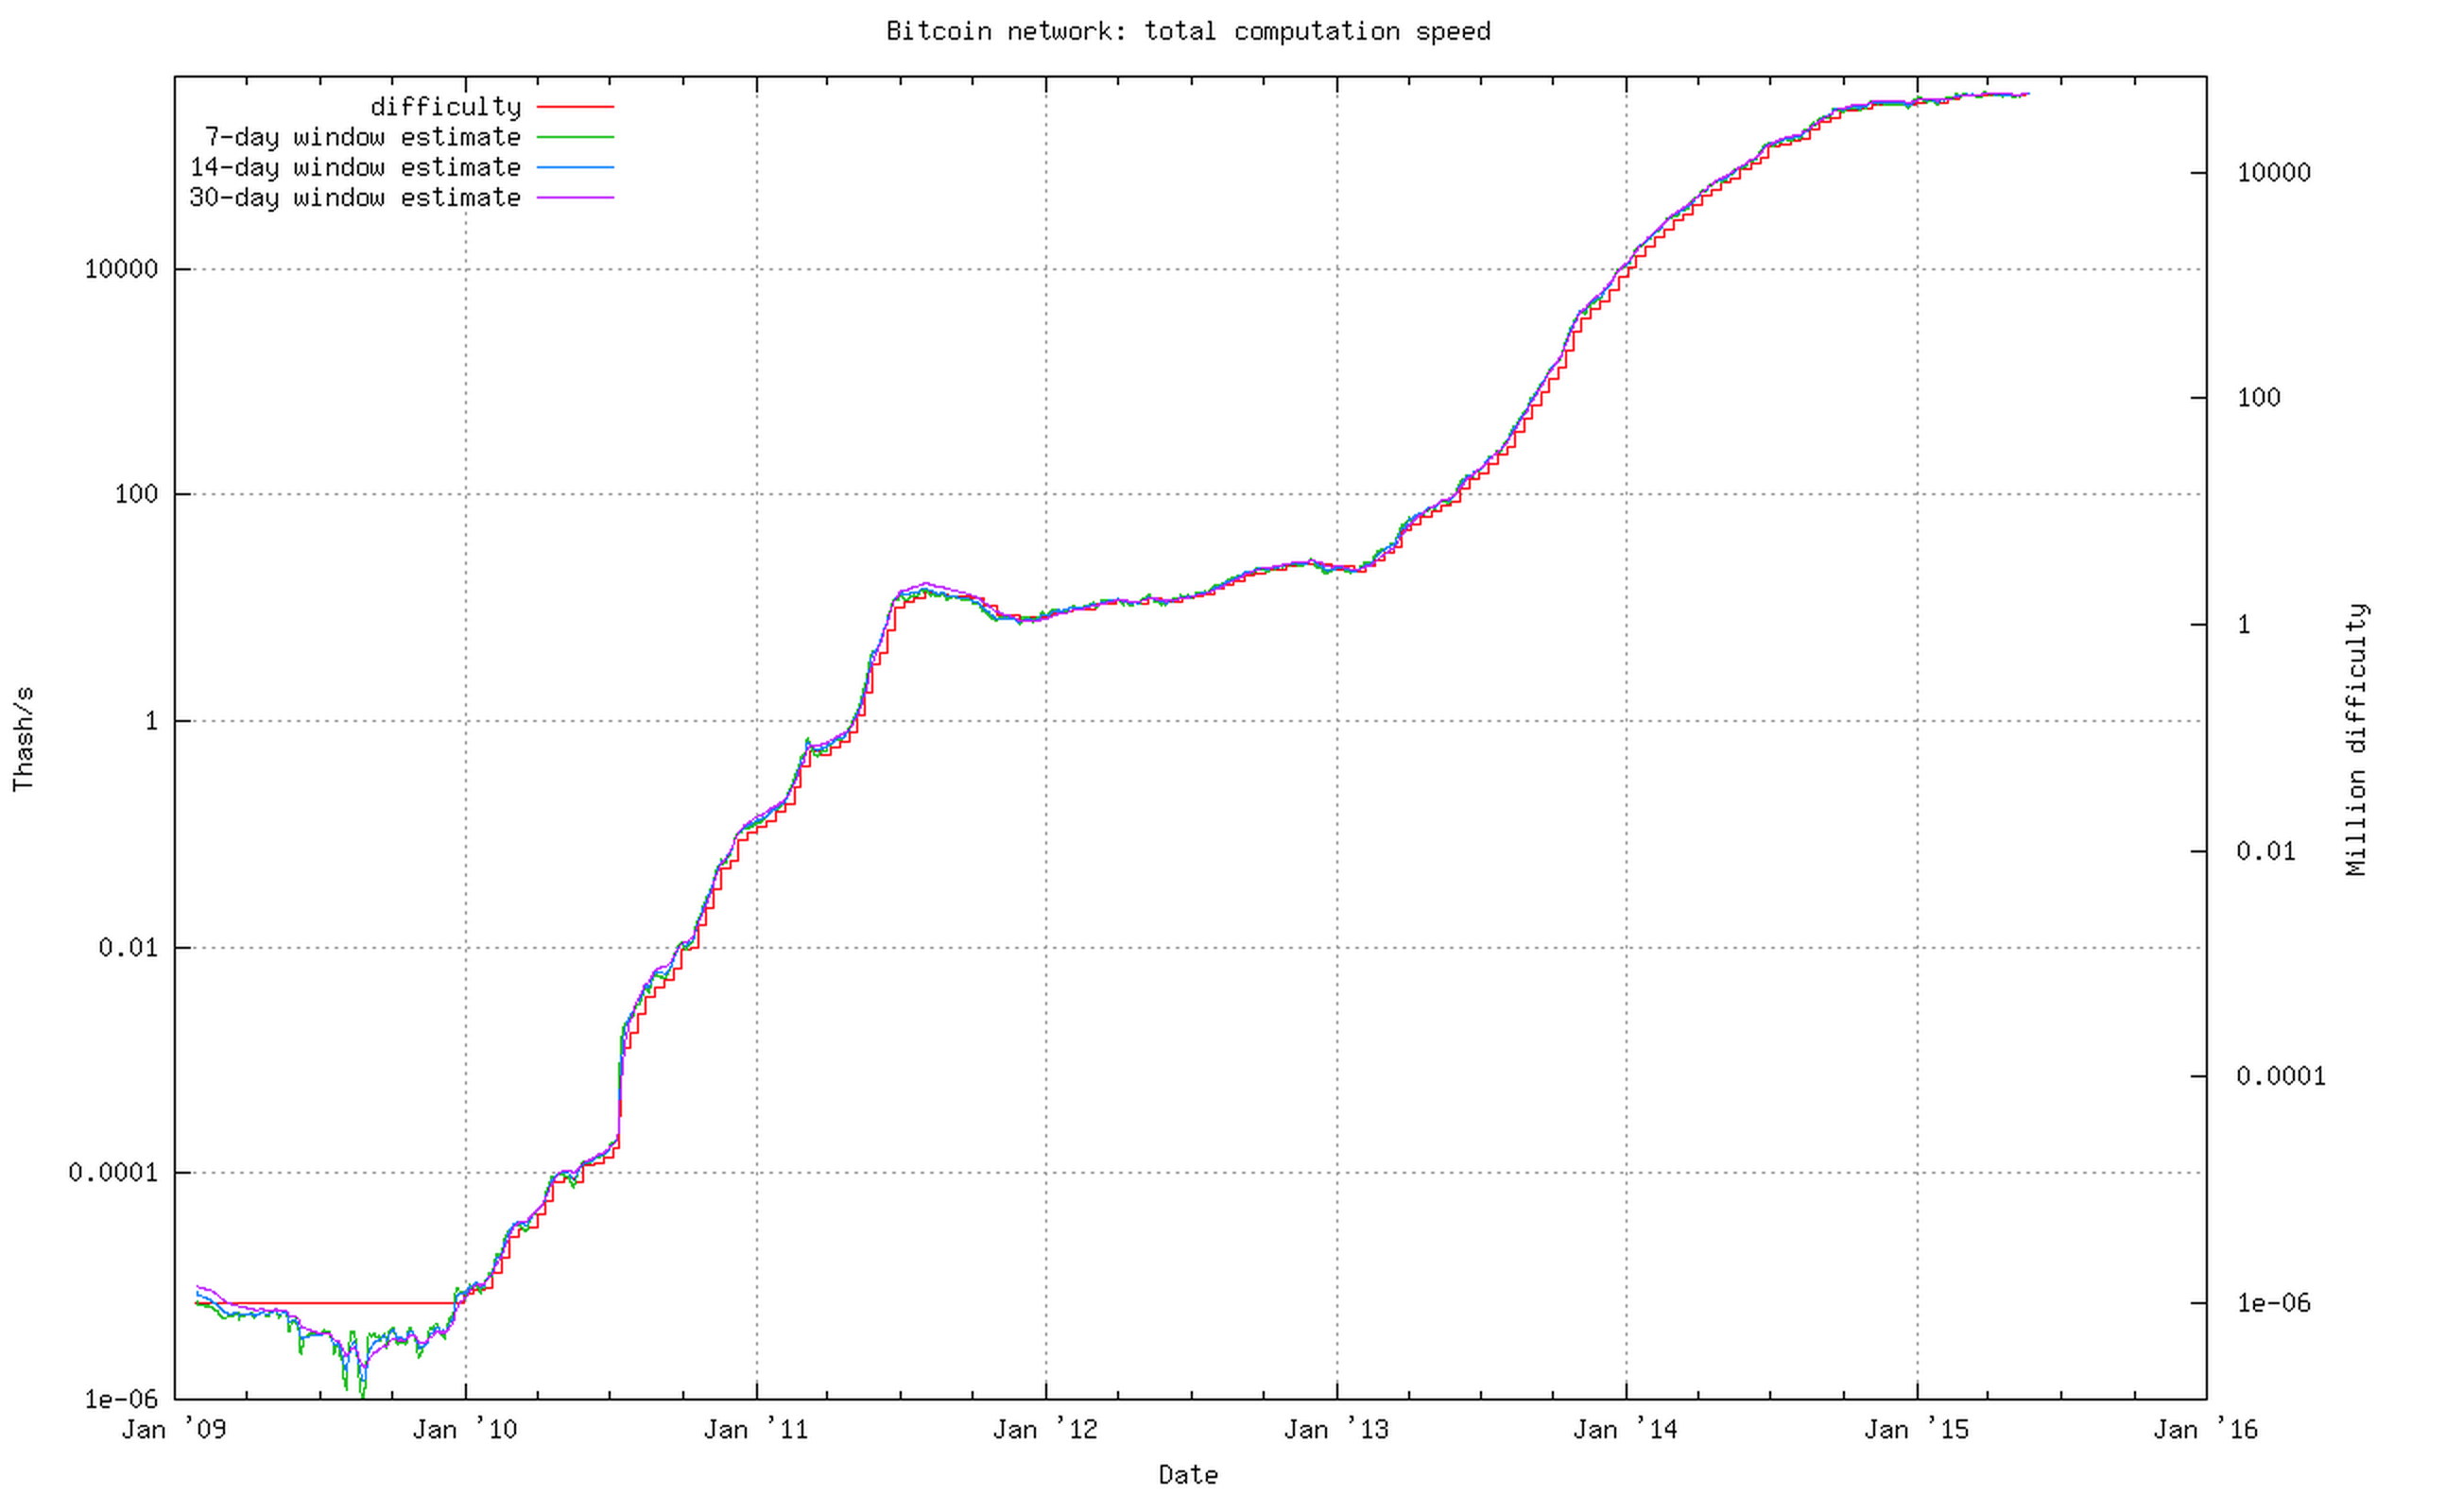
\includegraphics[width=0.95\textwidth]{Figures/Bitcoin/Difficulty-all}
%    \caption{The BTC Mining Difficulty, overall history from beginning until today.}
%    \label{fig:bitcoin-difficulty-all}
%\end{figure}
%
% COMMENTED OUT: TURNED OUT TO BE A DUPLICATE FROM EARLIER

\begin{figure}[htb]
    \centering
    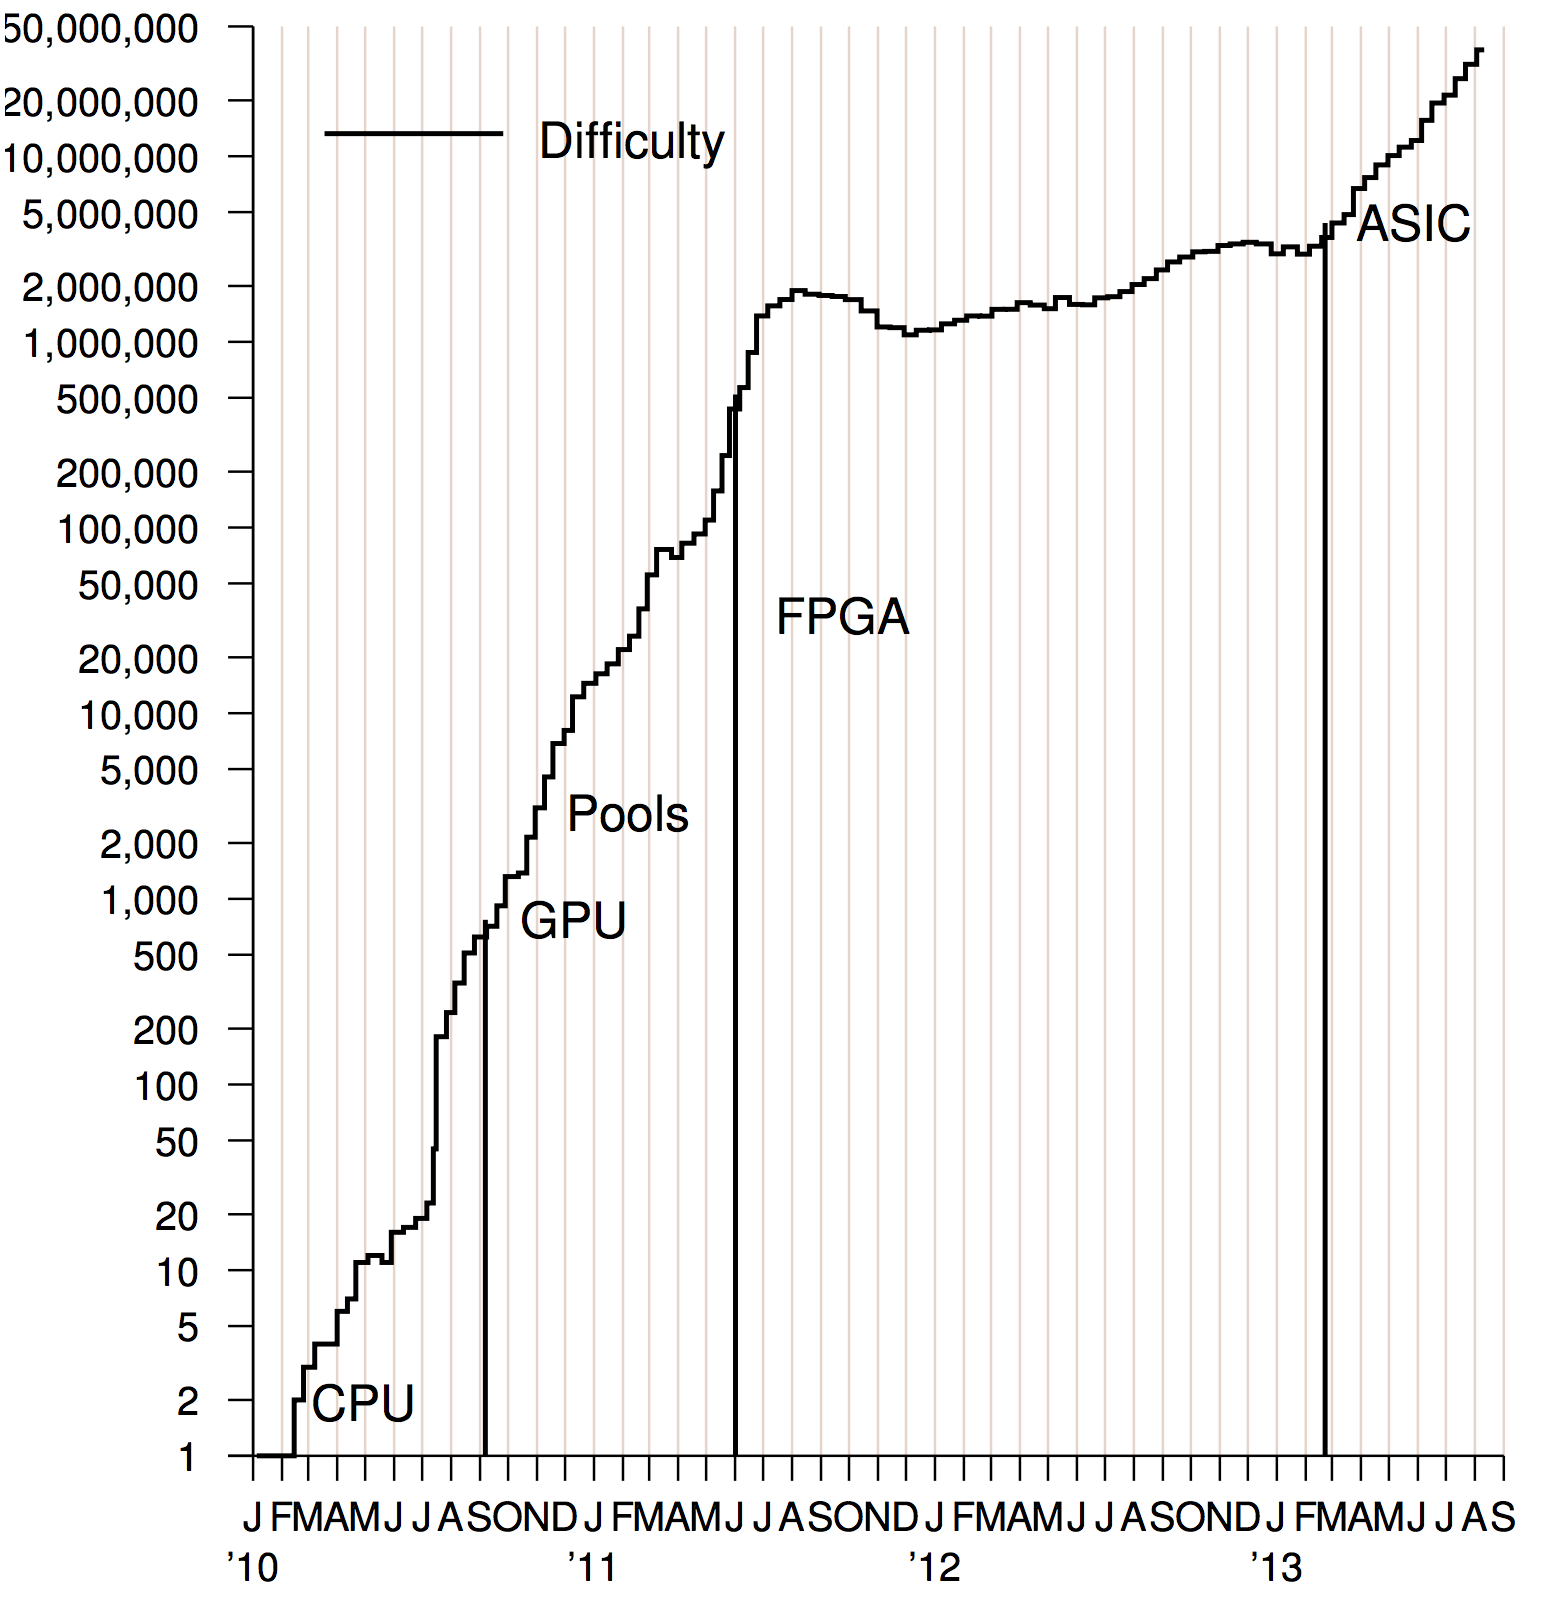
\includegraphics[width=0.95\textwidth]{Figures/Bitcoin/Difficulty-devices}
    \caption{The BTC Mining Difficulty, compared to when each generation was introduced, as seen in \cite{bespoke-silicon}.}
    \label{fig:bitcoin-difficulty-devices}
\end{figure}


%\textbf{Propose this chapter to replace "Bitcoin Hardware". Should not only contain the brief mentions of technology, but the way to achieve them, and lesson's learned underway (escially important for ASIC's having unexpected high energy use, and thus the way to the dark silicon area). Should end with going into dark silicon-problem.}
%
%\section{Existing Bitcoin Hardware}
%Due to bitcoin's popularity and the possibility of profits, various specialized hardware has been used
%to accelerate the process. Starting with simple programmes running on general-purpose processors,
%bitcoin miners soon turned to GPUs in order to improve the performance and power efficiency of the
%process. GPUs provide the possibility of running many hashing processes in parallel, in some cases
%exceeding 1 GH/s\cite{bitcoin-hardware-cmp}. FPGA-based bitcoin mining hardware provide
%better power efficiency than GPUs due to the possibility of tailoring the hardware design to
%bitcoin mining.\todo{Move to related work?}

%However, as bitcoin mining have become more profitable, ASIC-based bitcoin miners have taken over
%the market and currently dominates in terms of performance and power efficiency, with performance
%exceeding 200 GH/s \todo{reference http://www.spondoolies-tech.com/products/sp35-yukon-power-shipping-%from-stock}
%per chip\todo{Power?} \cite{bespoke-silicon}.

\section{Dark Silicon and Heterogenity}
\label{sec:dark-silicon}

Moore's law states that transistor density on integrated chips continue to double every
two years. In addition, native transistor speeds are increasing with a factor of 1,4.
According to Dennard scaling, which predicted that the power density of transistors, that
is the voltage and current used to operate the transistor, would scale down with the
size of the transistors, this would not be a problem; however, the energy efficiency
of transistors are only improving by a factor of 1.4, not keeping up with the scaling
of transistor size.

Under a constant power-budget, there is a shortfall of a factor of 2 in the energy budget,
and this utilization potential of a chip is falling exponentially by 2 times for each generation.
If the power limitation were to be based on the current generation, then designs would be 93,75\% dark in eight years.
This gives rise to the term ``dark silicon'', where a chip must either be underclocked or parts of
it turned off, giving rise to ``dark'' areas of the chip, in order to keep to a set power budget.
This is especially true for chips where the cooling solutions are no longer efficient enough to remove
the generated heat from a fully powered chip.

In order to work around this problem, the industry moved to using multicore processors around 2005.
However, adding multiple cores does not circumvent the problem in the long run.
Multicore chips will not scale as transistors shrink, and the fraction of a chip that can be filled with cores running at full frequency is dropping exponentially with each processor generation. 
Large fractions of the chip will be left dark - either switched off for a long time, or significantly underclocked.
Hence new designs are required, where new architectural techniques spend area to buy energy efficiency. \cite{dark-silicon}

\subsection{Approaches to the Problem of Dark Silicon}
\label{sec:taylor}

To work around the problem of dark silicon, several approaches have been suggested as solutions.
Taylor\cite{dark-silicon} have listed up four particular approaches: Shrinking the chip, dimming the chip, specialization and so-called "Deus Ex Machina".

%The need to work around the problem of dark silicon has lead to several approaches
%being suggested as solutions. In \cite{dark-silicon} Taylor describes a taxonomy called ``The four horsemen'',
%referring to the fact that none of the solutions appear to be ideal.
%These are four proposed responses that are emerging as solutions beyond making multicore chips \cite{dark-silicon2}.
%Taylor argues that future chips will apply not just one of these solutions, but all of them.
%It can be seen from the success of complex multi-regime devices like MOSFETs that engineering as a field has an enormous tolerance for complexity if the end result is better.

%The four horsemen are The Shrinking Horseman, The Dim Horseman, The Specialized Horseman and The Deus Ex Machina Horseman,
%each referring to a particular solution to the dark silicon issue. \cite{dark-silicon}

%\subsubsection{The Shrinking Horseman}
\subsubsection{Shrinking the chip}

Instead of having dark silicon on the chip, one may simply shrink the chip itself.
%Taylor\cite{dark-silicon} views these "shrinking chips" as the most pessimistic outcome.
Although all chips may eventually shrink somewhat, the ones that shrink the most will be those where dark silicon cannot be applied fruitfully to improve the product.
%\todo{Nært overflødig?}
These chips may rapidly turn into low-margin businesses for which further generations of Moore’s law provide small benefit.

Futhermore, there are other disadvantages: Exponentially smaller chips are not exponentially cheaper, since mask cost, design cost and I/O pad aread cannot be amortized. 
Competition will most likely favor chips that utulizes dark silicon to improve the overall product, causing chips that are only shrinked to sell at low market price, leading to loss for the company.
Exponential shrinking also leads to exponential rise in power density, and chip temperature will thus follow suit.
Meeting the temperature limit will increase the cost, at which the nominal scaling of energy efficiency is reduced below \todo{Feels weird}1.4X.
%Meeting the temperature limit will reduce the scaling below the expected energy effeciency, at the nominal \todo{Feels weird}1.4X scaling.

%There are also second-order effects assosiated with shrinking chips:

%\begin{itemize}
%    \item Exponentially smaller chips are not exponentially cheaper.
%    In addition to the silicon itself, cost include mask costs, design costs and I/O pad area.
%    These cannot be amortized, and the price will increase per mm$^2$, as the chip shrinks.
%    \item Shrinking the silicon can also shrink the chip selling price, but competition will likely force companies to utilize dark silicon if it can attain a benefit for the end product.
%    Companies who would rely on shrinking only, may loose the competition and sell chips at catastrophically decreased chip prices.
%    \item Exponential shrinking leads to exponential rise in power density, and chip temperature will thus follow suit.
%    Meeting the temperature limit will reduce the scaling below the nominal 1,4x expected energy efficienty. 
%\end{itemize}

%\subsubsection{The Dim Horseman}
\subsubsection{Dimming the chip}
While the fractions of dark transistors of the chip increases exponentially, the silicon area become exponantially cheaper as resource, relative to power and energy consumption.
This gives the opportunity to spend area to buy energy efficiency, and basing new architectures on this.
\todo{Consider adding a figure to better illustrate the point}Dark silicon area can be populated with logic that is used only part of the time.

The term "dim silicon" refers to use of general purpose logic that typically employs heavy underclocking or infrequent use, large amount of otherwise-dark silicon area are put to productive use while meeting the power budget.
The architecture has to strategically manage the chip-wide transistor duty cycle, to enforce the overall power constraint. 

The early 90-nm designs of, for instance, Cell and Prescott, were dimmed because actual power exceeded design-estimated power. 
Lately, more increasingly more elegant methods are converging, that make better trade-offs.
Among the dim silicon techniques are dynamically varying the frequency with the number of cores being used, scaling up the amount of cache logic, employing near threshold voltage (NTV) processor designs, and redesigning the architecture to accommodate bursts that temporarily allow the power budget to be exceeded, such as Turbo Boost and computational sprinting. \cite{dark-silicon}

% %\todo{This subchapter ended up long. Try to see if it can be reduced. Especially NTV}
%According to Taylor\cite{dark-silicon}, as exponentially larger fractions of a chip’s transistors become dark transistors, silicon area becomes an exponentially cheaper resource relative to power and energy consumption.
%Therefore new architectural techniques that spend area to buy energy efficiency is called for.
%Instead of shrinking silicon, one may consider populating dark silicon area with logic that is used only part of the time, and interesting new design possibilities occurs.
%The term "dim silicon" refers to techniques that put large amounts of otherwise-dark silicon area to productive use by employing heavy underclocking or infrequent use to meet the power budget.
%The architecture has to strategically managing the chip-wide transistor duty cycle to enforce the overall power constraint. 
%Whereas early 90-nm designs such as Cell and Prescott were dimmed because actual power exceeded design-estimated power, more increasingly more elegant methods are converging, that make better trade-offs.
%Among the dim silicon techniques are dynamically varying the frequency with the number of cores being used, scaling up the amount of cache logic, employing near threshold voltage (NTV) processor designs, and redesigning the architecture to accommodate bursts that temporarily allow the power budget to be exceeded, such as Turbo Boost and computational sprinting.

% %\todo{Consider shorting down or removing entire lists from each sub-chapter, to keep the four horsemen short and concise.}Amond dim silicon methods are: 

%\begin{itemize}
%    \item Turbo boost, where less core are active, the higher the frequency they may run at.
%    Energy gained from turning off cores is used to increase voltage and frequency of active cores.
%    This is known as Dynamic voltage and frequency scaling (DVFS).
%    \item Near-threshold voltage (NTV) Processors.
%    Transistors were at 2013 operated around 2,5x the threshold voltage, an energy-delay optimal point. 
%    This is at a point where reducing the voltage severely affects the frequency drop, which reduces the effective gain from downward-DVS.
%    Nevertheless, researchers have begun exploring this regime.
%    NTV logiv is a recent approach, where transistors in the near-threshold regime are operated slightly above the threshold voltage.
%    This provides a more palatable trade-off between energy and delay than subthreshold circuits, for which frequency drops exponentially with voltage decreases.
%    \todo{Give a proper mention of where the following numbers were taken from}
%    Although NTV per-processor performance drops faster than the corresponding savings in energy-per-instruction (5X energy improvement for an 8x performance cost), the perfor- mance loss can be offset by using 8x more processors in parallel if the workload allows it.
%    Then, an additional 5x processors could turn the energy efficiency gains into additional performance. 
%    \todo{Have to admit, I still don't understand how this is a gain. And this is almost the point of too much. Should remove the example, and find a different way to explain}So, with ideal parallelization, NTV could offer 5x the throughput improvement by absorbing 40x the area. 
%    But this would also require 40x more free parallelism in the workload relative to the parallelism consumed by an equivalent energylimited super-threshold many-core processor.
%    \item Bigger caches.
%    Because only a subset of cache transistors (such as a wordline) is accessed each cycle, cache memories have low duty cycles and thus are inherently dark. 
%    Adding cache is therefore one way to simultaneously increase performance and lower power density per square millimeter.
%    But the less memory-bound a running application is, the less the benefit.
%    \item Computational sprinting and turbo boost.
%    One temporarily exceeds the nominal thermal budget but relies on thermal capacitance to buffer against temperature increases, and then ramp back to a comparatively dark state.
%    These are used within "race to finish" computations.

%\end{itemize}

%\subsubsection{The Specialized Horseman}
\subsubsection{Specialization}
Instead of using general purpose logic, this approach focuses on specialized use of logic for selected tasks.
Within a set of processors, each are specialized for a subset of tasks, increasing energy efficiency or performance compared to a general purpose processor, for those particular tasks.
Any application are executed on the processor which is deemed as the most efficient.
Cores not in use are power- and clock gated, and thus do not waste energy unnecessarily.

Specialized accelerators already exist today that span diverse areas, including baseband processing, graphics, computer vision and media coding.
These enable orders-of-magnitude improvements in energy efficiency and performance, especially for computations that are highly parallel.
Systems with more coprocessors than general purpose processors is anticipated to rise, referred to as coprocessor-dominated architectures, or CoDAs.

Challenges with these systems are expected as well, one of them beeing the so-called "Tower of Babel" crisis.
The notion of general-purpose computation becomes fragmented, and the clear lines of communication between programmers and software and the underlying hardware is no more.
For instance, CUDA for NVidia GPUs cannot be used for similar architectures, such as AMD.
There are several cases of overspecialization problems between accelerators, so that they cannot be used for closely related classes of computaion.
New heterogenenous hardware is more difficult to adopt for third party programmers, due to the cost of programming heterogeneous (where a clear example is the \todo{Hint: Maybe look up more examples?}Sony PlayStation 3, compared to Microsoft XBox). 
Specialized hardware also risk becomming obsolete when standards are revised. \cite{dark-silicon}


%This is the use of dark silicon to implement a host of specialized processors.
%They can be more energy efficient, or much faster than a general purpose processor.
%Programs are executed where it is most efficient.
%Unused cores are power- and clock gated in order to keep them from wasting energy.

%Specialization is already being realized today in forms of specialized accelerators that span diverse areas such as baseband processing, graphics, computer vision, and media coding.
%These accelerators enable orders-of-magnitude improvements in energy efficiency and performance, especially for computations that are highly parallel.
%It is expected to see a rise of systems with more coprocessors than general processors.
%Tayler refers to them as coprocessor- dominated architectures, or CoDAs.

%One of the expected challenges it the so-called "Tower of Babel" crisis, as the notion of general-purpose computation is fragmented, and the traditional clear lines of communication between programmers and software and the underlying hardware is eliminated.
%For instance, CUDA for NVidia GPUs is not usable for similar architectures, such as AMD.
%Overspecialization problems between accelerators that cause them to become inapplicable to closely related classes of computation has been observed.
%In addition, adoption problems are also caused by the excessive costs of programming heterogeneous hardware (such as Sony Playstation 3 vs. Microsoft XBox), and there is always the risk that specialized hardware may become obsolete as standards are revised. \cite{dark-silicon}.

%\todo{The following sections are expanding challenges to the specialized horseman, beyond the basic. Consider carefully if this delves in too deply of our own project report, and delete it all if so.}
%The following challenges needs to be adressed:
%\begin{itemize}
%    \item To combat the "Tower of Babel" problem, it is required to define a new paradigm for how specialization is expressed and exploited in future processing systems. 
%    New scalable architectural schemas that employ pervasively specialized hardware to minimize energy and maximize performance are needed. At the same time they need to insulate the hardware designer and programmer from such systems’ underlying complexity.
%    \item  Amdahl’s law adds issues for specialization.
%    To save energy across the majority of the computation, broad-based specialization approaches that apply to both regular, parallel code and irregular code must be found.
%    It must also be ensured that communicating specialized processors doesn’t fritter away their energy savings on costly cross-chip communication or shared-memory accesses. 
%    \item Recent efforts. The UCSD GreenDroid processor. \todo{YEP!}Proposal: This is an example. Move and describe it in related works.
%\end{itemize}

%\subsubsection{The Dues Ex Machina Horseman}
\subsubsection{Dues Ex Machina}
The termology "Deus ex machina" comes from literature or theater, in which the protagonists seem increasingly doomed until the very last moment, when something completely unexpected comes out of nowhere to save the day.
In the case for dark silicon, one deus ex machina would be a breakthrough in semiconductor device technology.
The required breakthrough would have to be very fundamental, making it possible to build transistors out of devices other than MOSFETs. 
There are physical limits to what can be done with \todo{I chose to not elaborate this one further. Remove when delivering, unless we change our mind}leakage from MOFSET transistors, and transistors made of other devices may go beyond these limits.
New transistors must also be able to compete with MOFSETs in performance.
Tunnel field-effect transistors (TFET) and nanoelectromechanical system (NEMS) switches are examples on inventions that hint to order-in-magnitude improvements in the leakage problem, but they still fall short in performance.
Overall, this is the most unpredictable field of solution. \cite{dark-silicon}


%Taylor notes that this one is the most unpredictable\cite{dark-silicon}.
%He uses the termology "Deus ex machina" from literature or theater, in which the protagonists seem increasingly doomed until the very last moment, when something completely unexpected comes out of nowhere to save the day.
%In the case for dark silicon, one deus ex machina would be a breakthrough in semiconductor devices.
%The required breakthrough would have to be very fundamental, making it possible to build transistors out of devices other than MOSFETs. 
%There are physical limits to what can be done with \todo{I chose to not elaborate this one further}leakage from MOFSET transistors, and transistors made of other devices can combat this.
%New transistors must also be able to compete with MOFSETs in performance.
%Tunnel field-effect transistors (TFET) and nanoelectromechanical system (NEMS) switches are examples on inventions that hint to order-in-magnitude improvements in the leakage problem, but they still fall short in performance.

% Please rewrite the above, the word "horseman" is something we shouldn't use.

%\section{Heterogeneous Architectures}
%\label{sec:heterogeneous}
%\todo{Used as head chapter, but consider removal if SHMAC is the only heterogeneous computer described.}Heterogeneous multiprocessor contains of specialized processors for different classes of applications, and are the implementation of the specialization approach.
%One such system is the Single-ISA Heterogeneous MAny-core Computer (SMHAC), which is a research project 
initiated by EECS on NTNU. \cite{shmac-plan}

%\subsection{The Single-ISA Heterogeneous MAny-core Computer}
\section{The Single-ISA Heterogeneous MAny-core Computer}
\label{sec:shmac}
The Single-ISA Heterogeneous MAny-core Computer is an architecture for investigating heterogeneous systems at all abstraction levels, as illustrated in figure \ref{fig:shmacAbstractionLevels}.
%The point is to create a flexible framework in which different heterogeneous processors can be created from a collection of processing elements and accelerators. % - Not anymore?
The programming model is kept constant across SHMAC-instances, while the underlying implementation changes.
This way, software design space exploration is facilitated.
It implements a tile-based architecture with a mesh interconnect. All processor tiles implement the same
ARM ISA and the same memory model, in order to achieve a common programming model \cite{shmac-plan}.
An illustration of SHMAC can be seen in figure \ref{fig:shmac}.

\begin{figure}[htb]
    \centering
    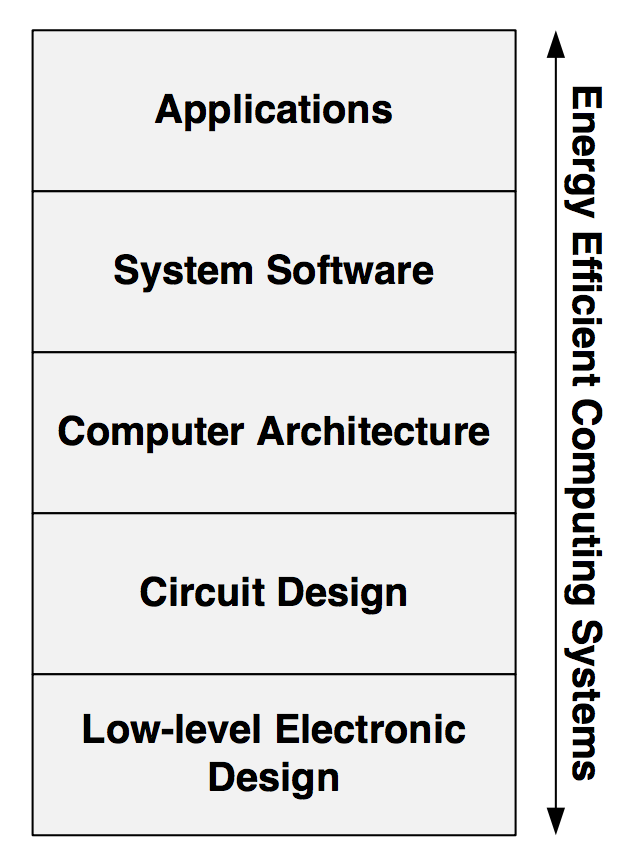
\includegraphics[width=0.5\textwidth]{Figures/Heterogeneous/SHMACAbstractionLevels}
    \caption{Levels of abstraction in computing systems \cite{shmac-plan}.}
    \label{fig:shmacAbstractionLevels}
\end{figure}

\begin{figure}[htb]
    \centering
    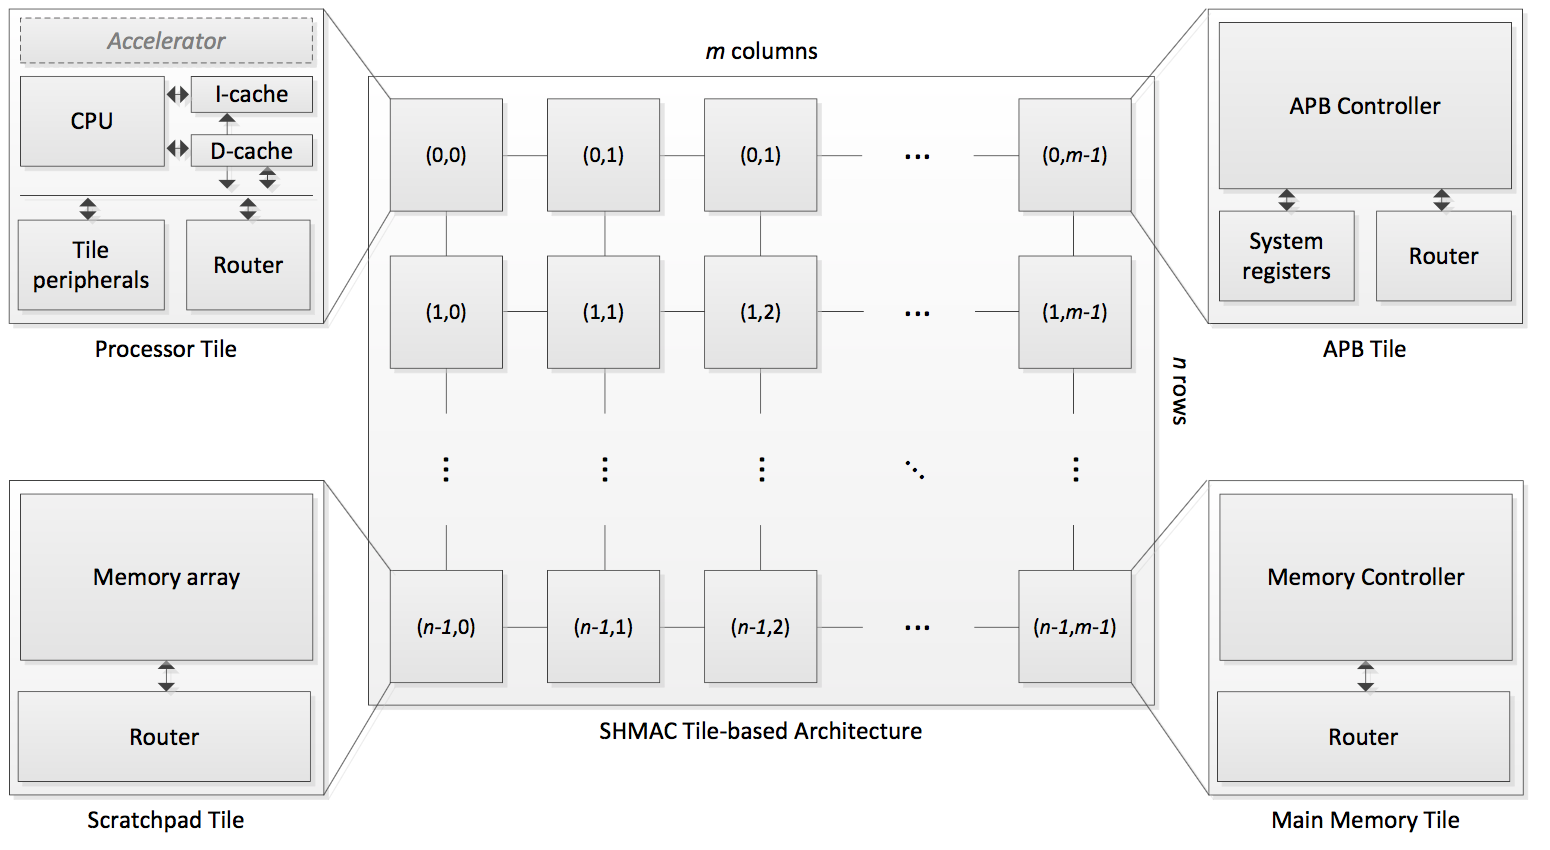
\includegraphics[width=0.95\textwidth]{Figures/Heterogeneous/SHMAC}
    \caption{High-Level architecture of SHMAC \cite{shmac-plan}.}
    \label{fig:shmac}
\end{figure}

%\todo{PROBLEM: This paragraph is way too similar to original text. Must fix, one way or another. }NTNU argues that the SHMAC-approach gives the right tools to reach the research goles outlined in the plan in \cite{shmac-plan}.
%For software research, SHMAC makes it possible to explore substantially more diverse systems than the ones currently provided by the industry.
%Furthermore, SHMAC-based computers realized in FPGAs will be significatly faster than using simulators.
%It is expected that co-developing software and hardware will result in new knowledge that gives insight into both hardware and software issues.
%Micro- and macro-architecture components can also be combined with novel transistor technologies and ASIC realizations to reach research goals at even lower abstraction levels.

% - Yes, I commented out this stuff: write what you want to say, then use citations to back it up - do not copy from the citations!

%We believe that the SHMAC-approach gives us the right tools to reach the research goals outlined in this plan. For software research, SHMAC makes it possible to explore substantially more diverse systems than those cur- rently provided by the industry. At the same time, SHMAC-architectures realized in FPGAs will be significantly faster than simulator-based approaches. We expect that co-developing software and hardware result in substan- tial cross-fertilization that gives insights into both hardware and software issues. Finally, the SHMAC micro- and macro-architecture components can be combined with novel transistor technologies and ASIC realizations to reach research goals at the lower abstraction levels.

%\subsubsection{SHMAC Architecture}
\subsection{SHMAC Architecture}

SHMAC is a tile-based architecture, with the processing elements laid out in a rectangular grid with neighbour-to-neighbour connection, using a mesh interconnect, using XY-routing.
%Several tile types are currently supported, not including the tile described in this report,
%with the most important ones being the processor tile, which contains a Turbo Amber CPU
%\footnote{See section \ref{sec:aht} for a short overview}, a scratchpad tile which functions as
%fast temporary storage, a DRAM tile and an I/O tile for communicating with a host system.

The supported tile types, not including the new tile described in this report, are the following:
\todo{Entire following list pretty much rip-off, except Amber and Turbo Amber. Sources from elsewhere needed.}
\begin{description}
  \item[Amber Processor Tile] The Processor tile that contains an ARM Amber processor, caches, peripherals and optional accelerators, and the general concept can be seen in figure \ref{fig:shmac-cpu}.
  \todo{Describe Amber Briefly}
  \textbf{Describe Amber Briefly}
  Currently, the peripherals consists of interrupt controller, timers and tile registers.
  The tile registers are per-tile memory that store local information like the processor ID, the coordinates of the tile, etc. 
  The caches, router and peripherals are connected to a Wishbone bus.
  
%  \todo{IMPORTANT! Affected our results!}Caches reduce the average memory latency, but adding caches also add the possibility for coherence problems.
%  This is currently solved by placing shared data in uncachable memory regions, through software. 
%  
  The processor tile can be equipped with optional accelerators, designed to execute a specified computation in a very effective way.
%  
%  
  \item[Turbo Amber Processor Tile] Same as previous, but has an ARM Turbo Amber processor with higher performance and runs the ARMv4nt instruction set. \cite{turboamber}
  \item[Scratchpad Tile] Includes memory and a router, but no processing element. 
  It is is an on-chip memory where the contents are managed by software (e.g. programmer, compiler, system software, etc.).
  Each scratchpad tile is given a 128 MB address space.
  The number of scratchpad tiles depends on a number of factors like the amount of block RAM available on the chosen FPGA, the desired access latency, the amount of block RAM used for caches in the processor tiles and the possibility of access contention\cite{shmac-plan}.
  The memory layout for SHMAC is seen in figure \ref{fig:shmac-memory}.
  \item[Main Memory Tile] Memory controller tile that gives SHMAC access to off-chip memory.
  \item[APB Interface] This tile implements the Advanced Peripherals Bus (APB) slave which gives the host processor on the Versatile boards access to SHMACs memory space. 
  In addition, the APB contains system registers which are used for managing communication with the host system.
  \item[Dummy Tile] Contains only a router and is used to fill remaining tiles when there is not enough resources available in the target FPGA to fill all tiles with tiles that implement functionality.\end{description}


\begin{figure}[htb]
    \centering
    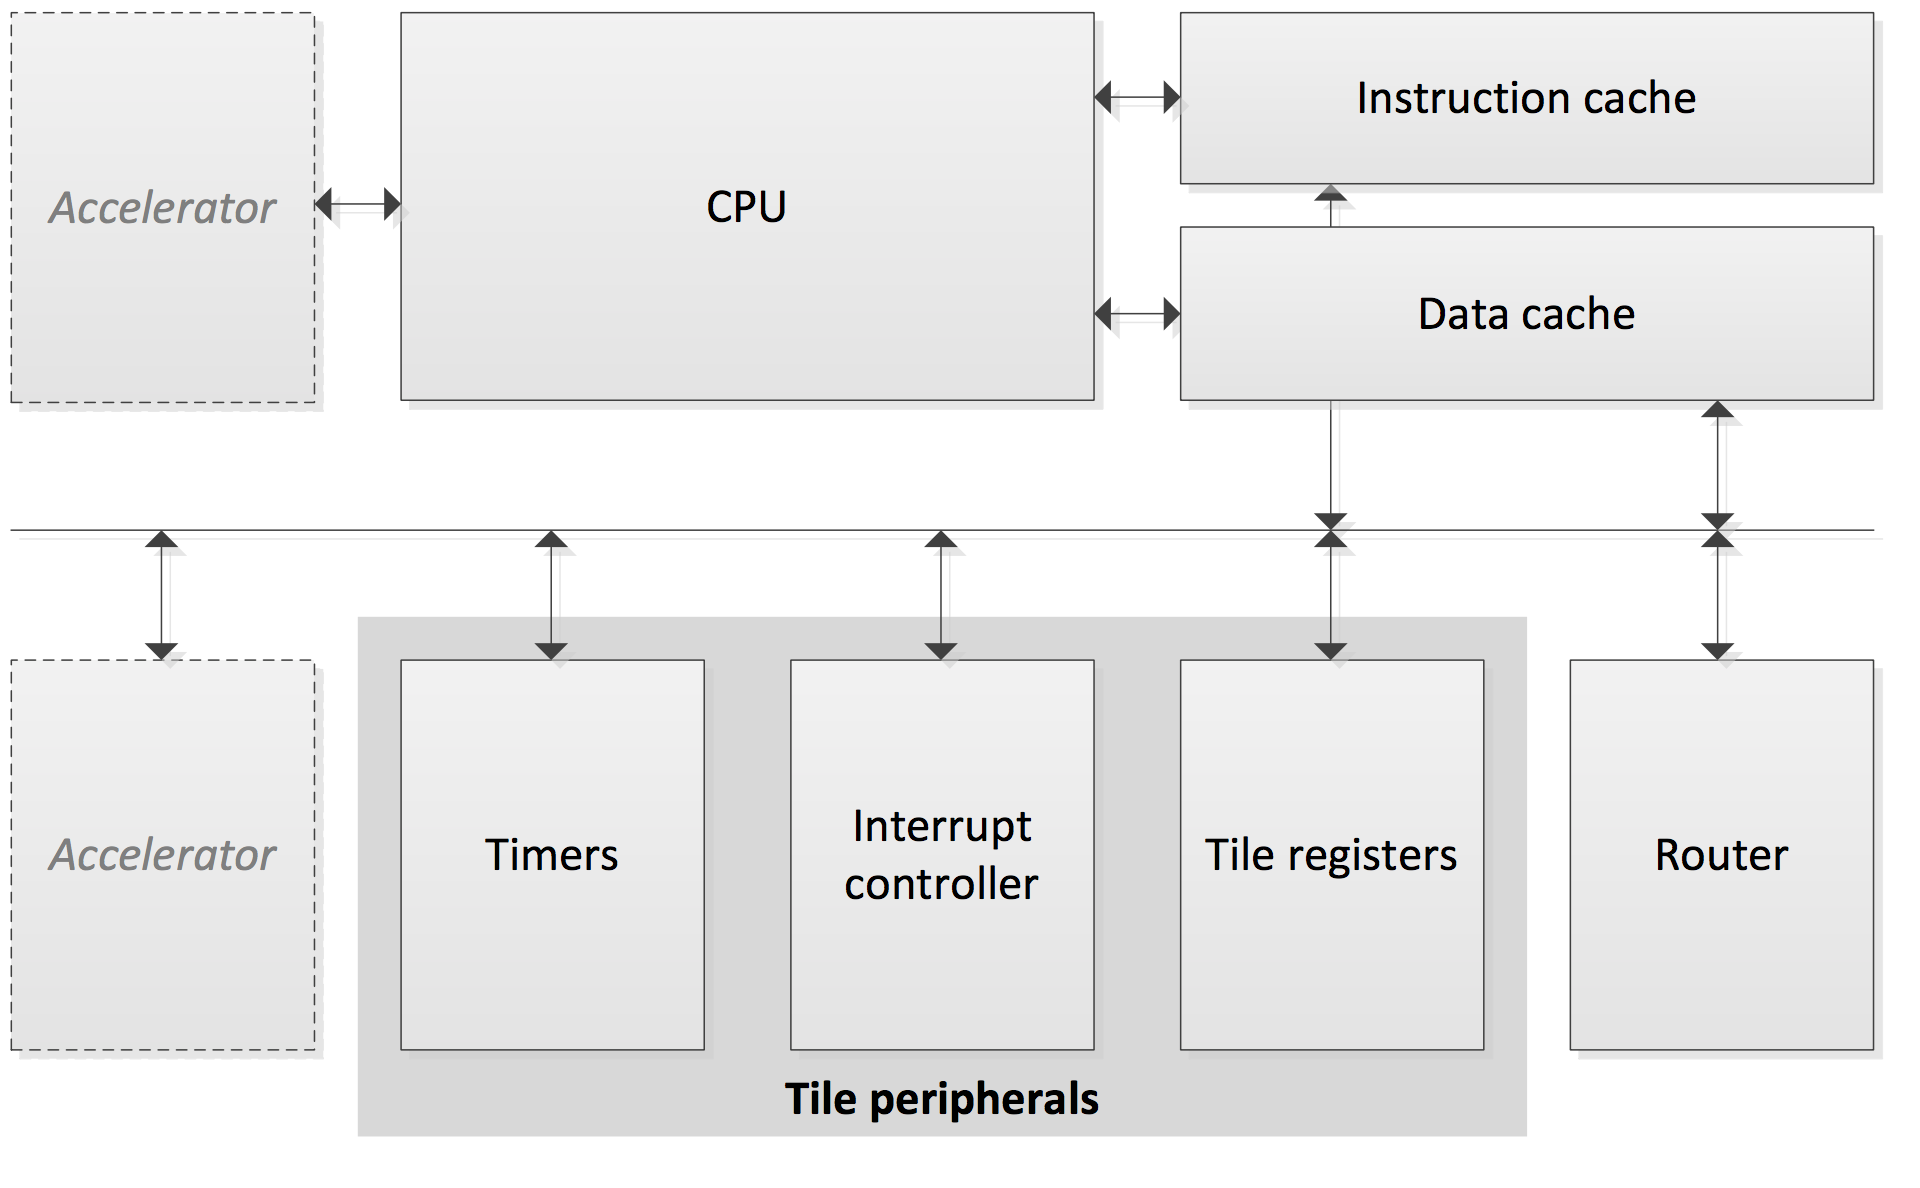
\includegraphics[width=0.8\textwidth]{Figures/Heterogeneous/SHMACCPU}
    \caption{SHMAC Processor tile \cite{shmac-plan}.}
    \label{fig:shmac-cpu}
\end{figure}

%\subsubsection{SHMAC Memory Map}
\subsection{SHMAC Memory Map}

%Figure \ref{fig:shmac-memory} shows how the memory is mapped in ARM-based SHMAC.
%
%The Exception table contains 8 instructions, one for each exception type described on \todo{Checked Redmine. Coulnd't find it}Redmine.
% NOTE: That is because it is standard ARM stuff, not SHMAC relevant - K.
%
The high end of the memory space is reserved for system registers and tile registers. 
The tile registers are private for each tile and contain information such as the tile's coordinates, CPU number and other useful data.
In addition the tile memory space contains the memory mapped peripherals for each tile, such as timers and the interrupt controller.
Any custom peripheral, such as the DMA and the hashing accelerator developed in the project is also mapped into this address space.
The system registers are used for communication with the host system.

%The scratchpad tiles have been given a 128 MB address space. The SHMAC architecture supports 1 to k scratchpad tiles where k can be chosen independently of the number of tiles in the SHMAC instance. The number of scratchpad tiles depends on a number of factors like the amount of block RAM available on the chosen FPGA, the desired access latency, the amount of block RAM used for caches in the processor tiles and the possibility of access contention.

\begin{figure}[htb]
    \centering
    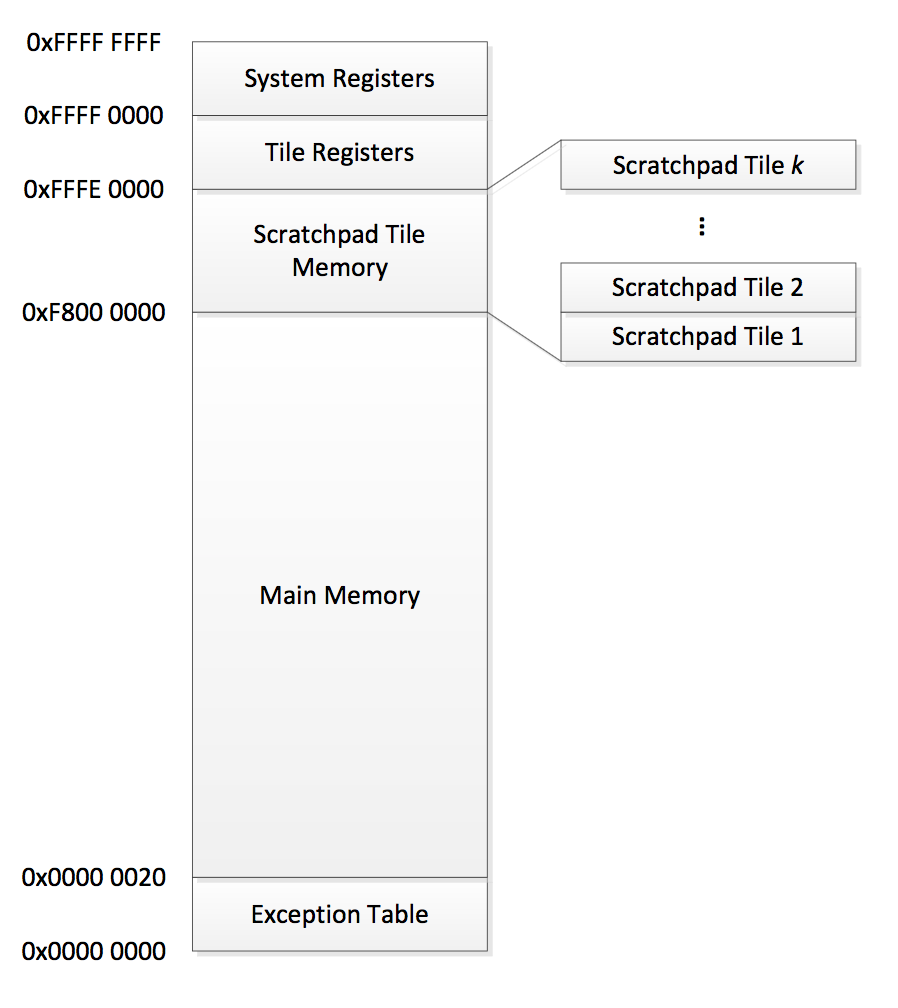
\includegraphics[width=0.6\textwidth]{Figures/Heterogeneous/SHMACMemory}
    \caption{Memory map of ARM-based SHMAC, as seen in \cite{shmac-plan}.}
    \label{fig:shmac-memory}
\end{figure}


%\subsection{Work packages}
%\textbf{Currently optional. Remove if nothing is worthwhile to mention. (LA STÅ)}

\subsection{SHMAC Interconnection Netwwork}
SHMAM uses a 2D mesh-based interconnection network to connect all the tiles.
Store-and-forward switching with on/off flow control is used, and the XY-algorithm is used for route computation.
Each tile consists of a router with five ports, for east, north, west, south and local connection, respectively.
A round-robin scheme is used, and packets from the local tile has equal priority to those arriving from the other directions.
In the current implementation, it takes 3 cycles for a data packet to transfer from one tile to the next. 
The architecture of the router can be seen in figure \ref{fig:shmac-router}.

\begin{figure}[htb]
    \centering
    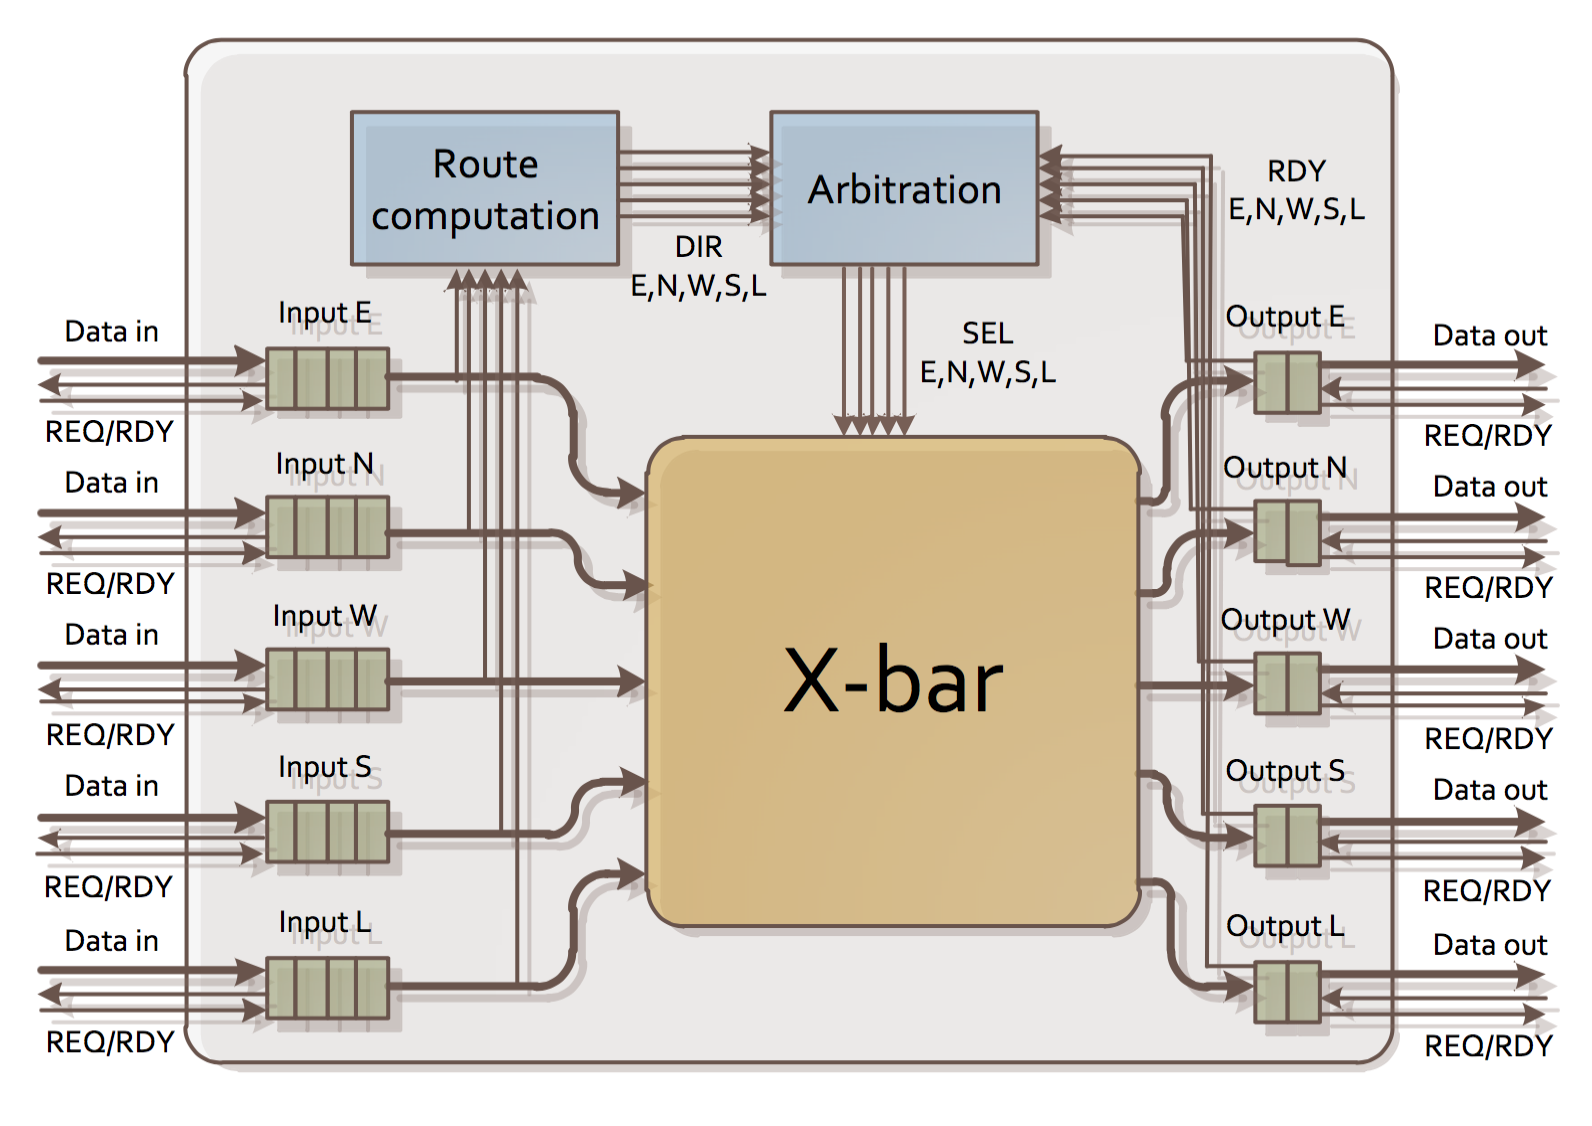
\includegraphics[width=1.0\textwidth]{Figures/Heterogeneous/SHMACRouter}
    \caption{Architecture of the SHMAC router, as seen in \cite{shmac-plan}.}
    \label{fig:shmac-router}
\end{figure}


%\section{SHMAC Network on Chip}
%\textbf{Optional position: Chapter 3 describing SHMAC}
%Write here the numbers from shmac: Expected tile-to-tile routing time, Max throughput on DRAM-access, etc.etc. Anything we know that may impact our testing of the bitcoin mining


%\subsection{SHMAC Performance}
%\section{SHMAC Performance}
%\textbf{Optional chapter position (if not in Methodology). DRAM throughput, routing speed, known costs, etc.}
%

\subsection{Wishbone Bus}
The WISHBONE SoC Interconnect Architecture was developed by OpenCores Organization as a flexible design methodology for use with semiconductor IP cores.
WISHBONE makes integration of IP cores more easy as it can be used as a common interface between IP cores, in contrast to using non-standard interconnection that requires custom "glue logic". 
This improves the portability and reliability of the system, and results in faster time-to-market for the end user.

\todo{Paragraph is rip-off. Write with own words. Or cut out}The WISHBONE architecture offers: a flexible integration solution that can be easily tailored to a specific application, a variety of bus cycles and data path widths to solve various system problems, and allow products to be designed by a variety of suppliers (thereby driving down price while improving performance and quality).

%NOTE: Added these details because they may be relecvant for "future work", especially concerning the DMA Module.
In the simplest implementation of WISHBONE, a WB master may request only one data transfer (either storing or loading) per transfer cycle, in which both the request and the cycles ends as soon as the request is acknowledged.
WISHBONE supports also burst mode, in which one cycle may consist of several transfers between the master and the WB slave.
Each request will last until acknowledged, before the WB master moves on to the next one.
Pipelining is also supported, in which the requests do not have to wait for acknowledge before ending, allowing multiple requests to be sent out before acknowledges arrive \cite{WISHBONE}.

WISHBONE is implemented as internal bus on the CPU tiles of SHMAC, but currently supports only single transfers with no bursts or pipelining.
This means that in spite of using switched packet interconnection network on SHMAC, something that opens up for sending out several packets, a WB Master on a tile will only send out one request, before getting the acknowledged response back.
\todo{Yaman said this. Find out if oral conversations with teachers/staff is allowed for bibliography.}\cite{Yaman}
And prior to this project, only one WB master existed on each tile, owning the entire WISHBONE network in the tile.

\subsection{Other properties of Vexpress}
FIND: DDR MEMORY LATENCY AND THROUGHPUT IF POSSIBLE.
Throughput according to Asbjørn: 128-bit word per cycle.
Clock is a 50MHz.

\section{Heterogeneous Processors}

Heterogenenous architectures offers various possibilities for improved performance and energy efficiency;
this could be in the systems ability to adapt to various applications or even external conditions such as
power or temperature conditions \cite{heterogeneous-ee, heterogeneous-perf, heterogeneous-arch}.

%Kumar \textit{et al} \cite{heterogeneous-ee, heterogeneous-perf, heterogeneous-arch} explores the diverse possibilities offered by heterogeneous architectures. 
%They prediction that core diversity will be of higher value than uniformity, and will offer much greater ability to adapt to the demands of the applications.
%They argue that the objective function can change over time, such as power conditions, application switches, or changes of demands within the application\cite{heterogeneous-ee}. 

\subsection{Energy Efficiency}
\label{subsec:rw_ee} 
Kumar \textit{et al}\cite{heterogeneous-ee} ran a simulation where they combined four generations from the Alpha family: EV4 (Alpha 21064), EV5 (Alpha 21164), EV6 (Alpha 21264) and a single-threaded version of EV8 (Alpha 21464), and made a heterogenous multi processor.
Only one application would run at the time, on one core, while the others were powered down.
The architecture, with the chosen cores and their relative sizes to one another can be seen in figure
\ref{fig:Kumar1}.

\begin{figure}[htb]
    \centering
    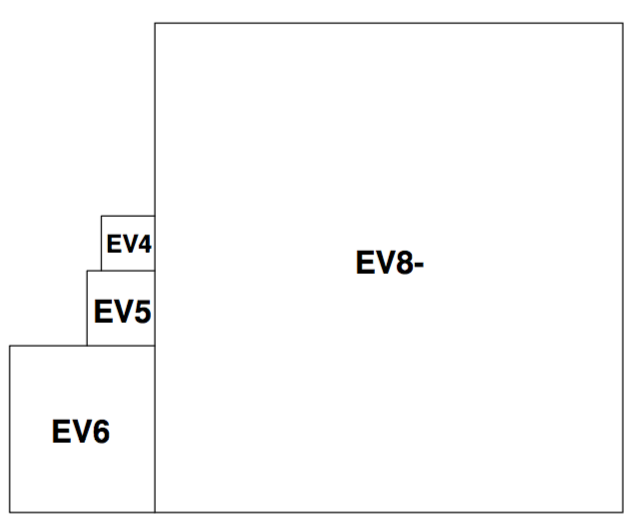
\includegraphics[width=0.5\textwidth]{Figures/Heterogeneous/Kumar1}
    \caption{Cores used in \cite{heterogeneous-ee}, and their relative sizes.}
    \label{fig:Kumar1}
\end{figure}


14 benchmarks from SPEC2000 were used in this experiment, simulated using SMTSIM, and both energy and energy-delay were measured.

For the simulation, it was assumed that the system knew the needs of every application, and selected core statically. 
Results showed average energy savings of 32\%, and average performance loss at only 2.6\%, relative to using the EV8 core.
Kumar \textit{et al} also used this experiment to show that dynamic core switching outperforms the best static core selection.
Simple heuristics would sample the cores at regular intervals, and execute core switch based on the results.
The heuristics achieved up to 93\% of the energy-delay gains compared to the best static selection. 

\subsection{Performance}
\label{subsec:rw_perf}
In another experiment, Kumar \textit{et al}\cite{heterogeneous-perf} proved that heterogeneity can be exploited to gain increased performance, for multithreaded workload.
They point out that heterogeneous architectures are advantagous for two reasons.

Firstly, they offer efficient adaptation to application diversity, as applications differs in their resource needs.
Some are compute intensitive and make good use of an out-of-order pipeline with high issue-width, while others may be memory-bound, and will underutulize advanced cores.
They may perform almost as well on an in-order core with low issue-width\cite{heterogeneous-perf}.

Secondly, heterogeneous architectures offers more efficient use of the die area for a given thread-level parallelism.
A complex core can be replaced by multiple smaller and simpler cores. 
Since the process or thread-level paralellism varies within most systems, a mix of cores that offers some large cores for high single-thread performce, and some small cores with high throughput per die area, is a potentially attractive area. \cite{heterogeneous-perf}

In contrast to the previous work described in \ref{subsec:rw_ee} by Kumar \textit{et al}, this experiment assigned multiple threads for multiple cores, and best global assignment was considered above best assignment for a selected application.
EV5 and EV6 from the Alpha family were chosen for this project, with one EV6 nearly equal to five EV5 in size.
With the total chip area anvailable for the architecture assumed to be 100 mm$^2$, the space could consist of maximum 4 EV6 cores, or 20 EV5 cores.
Three EV6 cores and five EV5 were chosen for this experiment, with expectation that it would perform well over a wide range of available thread-level parallelism. 
A small number from SPEC2000 benchmarks were chosen, with the focus on evaluating varying number of threads.
SMTSIM and Simpoint were used for the simulation.

%\todo{Mind-blowing, consider removal}Evaluation metric was weighted speedup, which in this context is the arithmetic sum of the individual IPCs of the threads constituting a workload divided by their IPC on a baseline configuration when running alone.
%In addition to performance gain, application response time within varying queue lengths is tested as well, to give insight on how well heterogeneous processors handles large queues, compared to best homogeneous systems.

Best static scheduling ensures that threads that are least affected by the difference between the EV5 and the EV6, are assigned to the EV5 processors, when all EV6 processors are occupied.
When the number of threads passes 4, the measured weighted speedup increases on the heterogeneous system, compared to a homogeneous CMP with 4 EV6.
When the number of threads passes 13, a CMP with 20 EV5 performs better, though this can be changed with a different combination of EV5 and EV6 cores.
This is shown in figure \ref{fig:Kumar2}.

%\todo{Following 2 sentences are nearly ripoff from \cite{heterogeneous-perf}, consider making quote or what?}
Compared to 4 EV6 cores, the heterogeneous processor performed up to 37\% better with an average 26\% improvement over the configuration considering 1-20 threads. 
Compared to 20 EV5 cores, the performance was up to 2.3 times better, and averaged 23\% better over that same range. \cite{heterogeneous-perf}
Using dynamic heuristics for core assignment further increased the performance.

\begin{figure}[htb]
    \centering
    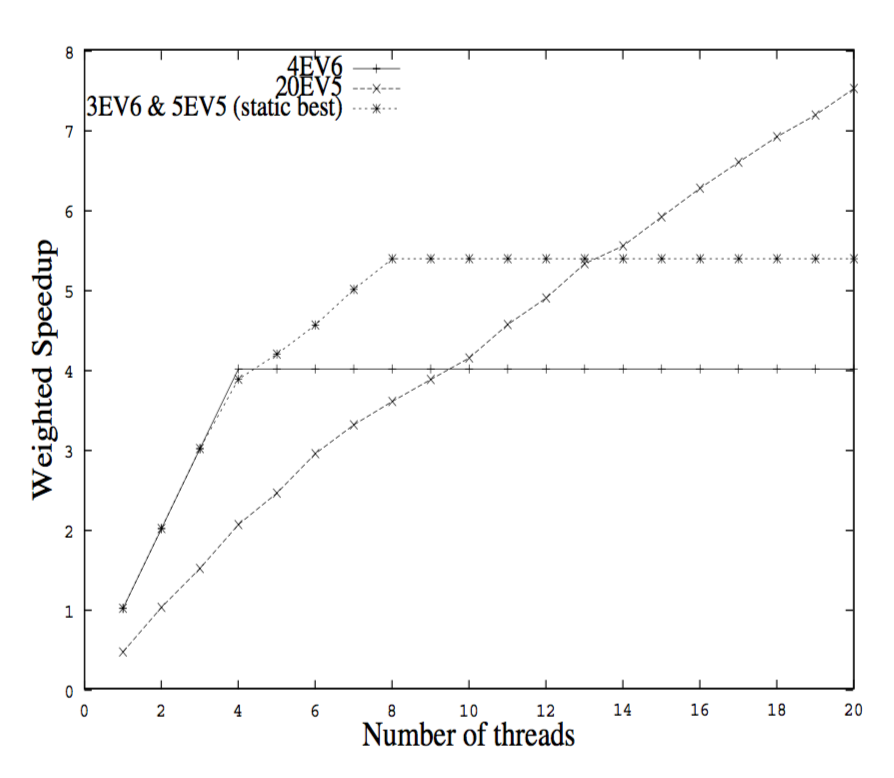
\includegraphics[width=0.5\textwidth]{Figures/Heterogeneous/Kumar2}
    \caption{Benefits from heterogeneity - static scheduling for inter-thread diversity, as seen in \cite{heterogeneous-perf}.}
    \label{fig:Kumar2}
\end{figure}

In addition to testing the performance gain, Kumar \textit{et al} also tested the the response time within queue lenght as well.
This was to give insight on how well heterogeneous processors handles large job queues, compared to best homogeneous systems.
%For testing response time in an open system, and how various que length affects it, jobs with an average distrubition of 200 million cycles were generated randomly and executed.
For this test, jobs with an average distrubition of 200 million cycles were generated randomly and executed.
Then different mean job arrival rates with exponential distribution were simulated.
It was revealed a great difference between saturation for a homogenous system with 4 EV6, and the heterogeneous processor.
For the former, the unbounded response time is seen as the arrival rate approached its maximum throughput around 2 jobs per 100 million cycles.
From there, the run queue became infinate.
The heterogeneous system remained stable well beyond that point.
The degredation was also more graceful under heavier loads than for homogeneous processors.
This can be seen in figure \ref{fig:Kumar3}.

\begin{figure}[htb]
    \centering
    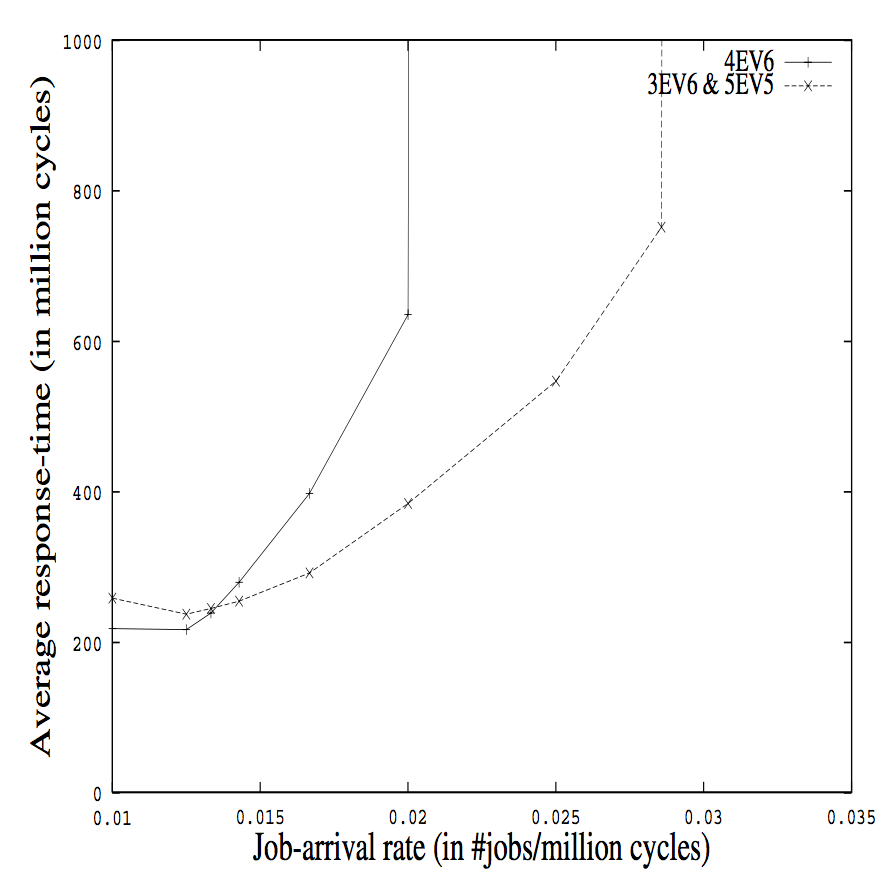
\includegraphics[width=0.5\textwidth]{Figures/Heterogeneous/Kumar3}
    \caption{Limiting response-time for various loads, as seen in \cite{heterogeneous-perf}.}
    \label{fig:Kumar3}
\end{figure}

\subsection{Optimal architecture}
\todo{Subchapter needs double check against source papers}
\label{subsec:rw_arch}
Kumar \textit{et al}\cite{heterogeneous-arch} has taken a closer look at what is good heterogeneous design.
They argue that while the previous experiments gave increased energy efficiency and performace, a heterogeneous system should be designed from scratch, instead of using pre-existing core designs.
While they surpassed homogeneous designs, pre-existing cores failed to reach the full potential of heterogeneousy for three reasons: They present low flexibility in choices, the core choices remain monotonic, and best heterogeneous design are composed of specialized core architectures\cite{heterogeneous-arch}.
But also, if pre-existing cores are not used, additional costs in design, verification and testing must be evaluated, to see if the benefits are worth the cost.

They made three significant contributions in this experiment. 
First, benefits of heterogeneity in power and area efficient architectures is re-evaluated, with new benefits and higher gains shown.
Secondly, methodologies for for arriving at good heterogeneous designs are demonstrated.
Thirdly, a number of key principles critical to effective design of future chip multiprocessors are identified.

Several conclusions were derived:
%\todo{Itemize or cut down at this point}
The most efficient heterogeneous multiprocessors were not constructed from cores that make good general-purpose uniprocessor cores, or cores that would appear in a good homogeneous multicure architecture.
Each core was individually tuned for a class of applications with common characteristics.
The results are usually non-monotonic processors.
And performance advantages of heterogeneous multiprocessors, including non-monotonic also holds for completely homogeneous workloads.
In those cases, the diversity across different workloads are exploited.

%\todo{Just a headnote. Remove when agreed or fixed}\textbf{Simplification assumptions dropped}

%A number of 480 unique cores could be made from the various parameters set for this experiment.
%\todo{Makes absolutely sense at all. Cut down or delete, but some way explain what the parameters were.}These were the issue width, I-cache size, D-cache size, L2 Cache size, Memory Channel, number of FP-IntMul-ALU units, IntQ-fpQ and IntFp PhysReg-ROB (OOO), ITLB-DTLB and LD/St Queue.
%\todo{Mention the "best fit" problem from monotonic cores?}
%\textbf{Insert mentioned todo-content or remove. And find suitable place}

A fixed number of four cores were used for this experiment.
In addition to testing the various core builds, the combinations were tested against varying area and power constraints, with their performance compared to the best homogeneous multiprocessors.
Static mapping were mainly used for this experiment, but few tests with dynamic mapping showed further increase in performance, since a thread could be moved around to most suitable core at any phase of its execution. 

%\todo{Strongly considering deleting (commenting out) the following paragraph. Too much unnecessary details.}The workloads come from seven benchmarks from the SPEC suite, classified int o processor bound or bandwidth bound.
%The chosen benchmarks are carefully selected, and represents the entire SPEC suite.
%In additional, three other benchmarks from other suites are chosen as well.
%Every multiprocessor is evaluated on two classes of workloads, called \textit{all different} and \textit{all same}.
%\todo{Warning: Direct rip-off. Consider "quote"-form}The former consist of all possible 4-threaded combinations that can be constructed such that each of the 4 threads running at a different time.
%The latter consists of all combinations that can be constructed so that all the 4 threads running at a time are the same.

%\todo{Direct copy, rewrite the paragraph}We use weighted speedup [21] for our evaluations. In this paper, weighted speedup measures the arithmetic sum of each running thread’s IPC, divided by its IPC on the simplest core considered in this study when running alone. The IPC is derived by running a thread for a fixed amount of time. We believe that this metric guards against multiprocessor design points that produce artificial speedups by simply favoring high-IPC threads.
%For completeness reasons, we also performed all our evaluations for total IPC as well and found that while the absolute results were different, there was no significant difference in trends or analysis.

It turned out that the more constricted the anvailable power or chip area, the more gain custom heterogeniety provided, as homogeneous multiprocessors could only perform any task at maximum if the power budget was generous.
But as designs become more aggressive, one will want to place more cores on the die, and power budgets per core is likely to tighten more severly.
Heterogeneous designs dampen the effects of constrained power budgets \cite{heterogeneous-arch}.

Any best heterogeneous design for the different tested power and area constraint were very different from best homogeneous design, underlining the need to design heterogeneous processors from a clean slate, rather than modifying an existing core design.
Monotonous designs (for instance, different generations of cores from same family) does not exploit heterogeneity equally well.
For instance, the benchmark \textit{mcf} from \cite{heterogeneous-ee} were mapped on EV6 or single-threaded EV8-, in spite of having low ILP.
The reason was the larger caches of these cores, causing the advances capabilities of these larger cores to be underutulized.

Heterogeneous multicore processors designed from clean slate gives better performance.

%\subsection{Uncore}
%\todo{Client worklod description has been cut out. Reconsider if it should be included}
%\label{subsec:rw_uncore}
%Gupta \textit{et al}\cite{heterogeneous-uncore} ran experiments with a heterogeneous multiprocessor, with the goal of measuring the impact of "uncore" power on the energy efficiency of heterogeneous multicore processors.
%In this experiment, they focused on the use of client devices, where energy is a premium resource and the workload profiles are diverse.
%The uncore is a collection of components of a processor, not in the core, but essential for core performance.
%Some of these components are the last level cache (LLC), integrated memory controllers (IMC), on-chip interconnect (OCI), power control logic (PWR), etc.
%With growing cache size and integration of various SoC components on the CPU die, the uncore is becoming an increasingly imporant contributor \cite{heterogeneous-uncore}.

%If a core has varying levels of sleep states, where the "deeper the sleep", the less power used, then uncore will be as active as the most active core.
%If three cores are idle (or on low activity), and one core is on highest activity, then the uncore will be on the highest activity.
%If for a task, the choice is between a big fast core, or a more power efficient small core, and the small core is chosen, the ucore will stay active for longer time, impacting the possible energy saving.
%This can be seen illustrated in figure \ref{fig:Uncore1}.

%\begin{figure}[htb]
%    \centering
%    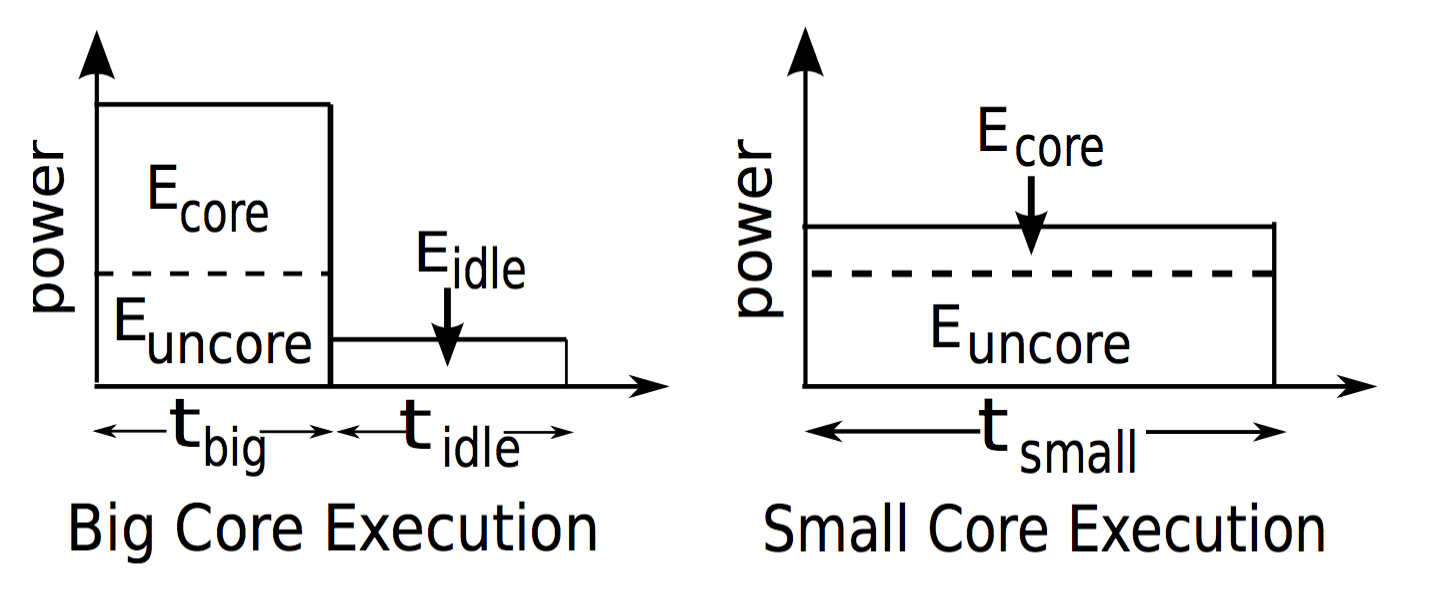
\includegraphics[width=1.0\textwidth]{Figures/Heterogeneous/Uncore1}
%    \caption{Effect of uncore power on the energy efficiency of heterogeneous cores, as seen in \cite{heterogeneous-uncore}.}
%    \label{fig:Uncore1}
%\end{figure}


%\todo{WARNING}\textbf{Skipped client workload description}

%The analysis considered two uncore conficurations: fixed and scalable.
%The first one used the same uncore subsystem for both big and small cores.
%The second modeled an uncore where certain components were turned off or powered down when moving to small cores.
%Examples are fewer memory channels, controllers, or smaller caches used.  

%\begin{figure}[htb]
%    \centering
%    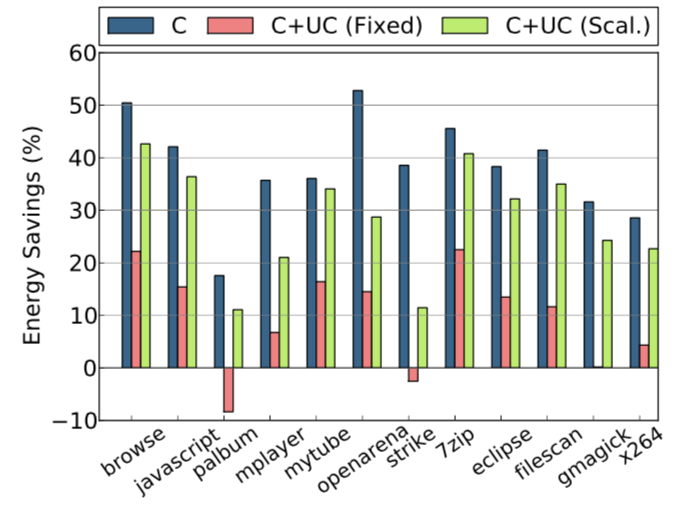
\includegraphics[width=1.0\textwidth]{Figures/Heterogeneous/Uncore2}
%    \caption{Energy savings of using small cores, with core-only savings (C), and with SoC-wide savings (C+UC), with a fixed uncore, and with a scalable uncore, as seen in \cite{heterogeneous-uncore}.}
%    \label{fig:Uncore2}
%\end{figure}

%Figure \ref{fig:Uncore2} shows the energy saved when going from big to small core, with both fixed and scaled uncores.
%It is clear that without scaling of the uncores, energy saving is reduced, even wasted in some cases.
%Figure \ref{fig:Uncore3} shows the relative contribution of core and uncore energy consumption for all the applications during big core execution, on a fixed uncore configuration.

%Clearly it is important to take uncore power into account for scheduling operations, and design of scalable uncore design is motivated, to obtain better gains from heterogeneous multicores. 

%\begin{figure}[htb]
%    \centering
%    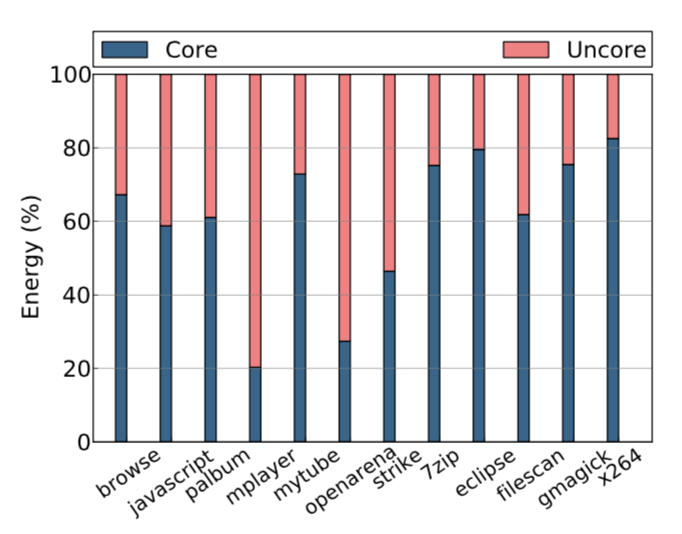
\includegraphics[width=1.0\textwidth]{Figures/Heterogeneous/Uncore3}
%    \caption{Core and uncore energy contricution for big cores and fixed uncores, as seen in \cite{heterogeneous-uncore}.}
%    \label{fig:Uncore3}
%\end{figure}

\section{Heterogenity and Bitcoin Mining}

Because of the need for all available computing power to solve hashes, heterogeneous architectures
may not seem the best solution for 

Heterogeneous systems may be configured to include bitcoin mining as an application. This can be
done by either making a complete, separate bitcoin mining core in a heterogeneous computer
or by incorporating an accelerator into an existing core or as a peripheral in such a system.

The Zedboard is a platform using a Zynq-7020 system-on-chip from Xilinx, which consists of
two Cortex-A9 processors, various peripherals and an FPGA area. This platform was evaluated
as a possible bitcoin mining platform, by using a separate bitcoin mining
accelerator. The accelerator included hardware for accelerating both the double SHA-256 calculation
and for comparing the result with the target value. At 50 MHz they obtained a performance of about
0.8~MH/s. \cite{xcell-bitcoin,standridge-master}



